\qns{An Introduction to Bode Plots}
\qcontributor{Justin Yu, Taejin Hwang}
\pgfplotsset{compat=1.9, every tick label/.append style={font=\normalsize}} 

Bode plots provide us with a simple and easy tool to plot these transfer functions by hand. \textbf{Always remember that Bode plots are an approximation}; if you want the precisely correct plots, you need to use numerical methods (like solving using MATLAB or IPython).

When we make Bode plots, we plot the frequency and magintude on a logarithmic scale
and the angle in either degrees or radians. We use the log scale because it allows us to break up complex transfer functions into its constituent components. 

We note that every transfer function can be written in its \textit{rational transfer function form,} which is a product of poles and zeros. When making the Bode plot (and plotting using a logarithmic unit), we treat each individual pole and zero independently, and then add them back together at the end. This question will examine the Bode plots of single zeros and poles, and we can generalize these plots to create a Bode plot for any transfer function.

\begin{enumerate}

\qitem Let's start by taking a look at $H(\omega) = X(\omega)Y(\omega)$, the product of two transfer functions $X$ and $Y$.
\begin{enumerate}
    \qitem How can you graph $|H(\omega)|$ using the graphs of $|X(\omega)|$, $|Y(\omega)|$?
    \qitem How does this compare when graphing $\log |H(\omega)|$ using the graphs of $\log |X(\omega)|$, $\log |Y(\omega)|$?
    \qitem What is the relationship between $\angle H(\omega), \angle X(\omega),$ and $\angle Y(\omega)?$
\end{enumerate}

\sol{
\begin{enumerate}
  \qitem To get $H(\omega),$ we would have to multiply the graphs of $|X(\omega)|$ and $|Y(\omega)|.$
  \qitem Since $\log |H(\omega)| = \log |X(\omega)| + \log |Y(\omega)|,$ we would have to add the graphs of $\log X(\omega)$ and $\log Y(\omega)$ which is much easier to do.
  \qitem $H(\omega) = |H(\omega)| e^{j \angle H(\omega)} = |X(\omega)| e^{j \angle X(\omega)} \cdot |Y(\omega)| e^{j \angle Y(\omega)} = 
  |X(\omega)| |Y(\omega)| e^{(\angle X(\omega) + \angle Y(\omega))}.$ \\
  Therefore, $\angle H(\omega) = \angle X(\omega) + \angle Y(\omega).$
\end{enumerate}
}

\qitem Let $H_z(\omega) = 1 + j \frac{\omega}{\omega_z}$. This is called a \textbf{zero at $\omega_z$}, where $\omega_z$ is the \textbf{zero frequency}.
\begin{enumerate}
    \qitem \textbf{Find $|H_z(\omega)|$ and $\angle H_z(\omega)$.}
           \textit{Hint: Consider the geometric interpretation of the transfer function as a complex number.
           Calculating the magnitude and angle is the same as in standard Cartesian coordinates.}
    \qitem Bode plots are approximations to the true transfer function, which means we only need to analyze the behavior in a few regions to sketch out an approximation to any transfer function's behavior.
    Typically, we will analyze the behavior at three regions: $\omega << \omega_z$, $\omega = \omega_z$, and $\omega >> \omega_z$.
    \textbf{Fill in the following table for the values of $|H_z(\omega)|$, $|H_z(\omega)|$, $\angle H_z(\omega)$ at these regions:}

    \begin{table}[h]
      \centering
      \begin{tabular}{| l | >{\centering\arraybackslash}m{6em} | >{\centering\arraybackslash}m{6em} | >{\centering\arraybackslash}m{6em} |} 
      \cline{2-4}
      \multicolumn{1}{l|}{}& $\omega << \omega_z$ & $\omega = \omega_z$ & $\omega >> \omega_z$ \\
      \hline
      &&&\\
      $H_z(\omega)$        &                      &                     &                      \\
      &&&\\
      \hline
      &&&\\
      $|H_z(\omega)|$      &                      &                     &                      \\
      &&&\\
      \hline
      &&&\\
      $\angle H_z(\omega)$ &                      &                     &                      \\
      &&&\\
      \hline
      \end{tabular}
    \end{table}

    \qitem \textbf{Plot the Bode plot for $|H_z(\omega)|$ and $\angle H_z(\omega)$ using the log-log plots below with $\omega$ on the x-axis.} (\textit{Sanity check: Why are we using log-log plots?})

    \begin{quote}
    \textbf{Note:} To plot these log-log plots using the values we calculated in the table above, we approximate the point $\omega << \omega_z$
    to be at $\omega = \frac{\omega_z}{10}$ and the point $\omega >> \omega_z$ to be at $\omega = 10\omega_z$.
    These differ from the zero frequency by a factor of 10 because we are using a base 10 log-log plot. \textbf{Plot the 3 points calculated above and connect them with straight line approximations.}
    \end{quote}

\end{enumerate}

\begin{figure}[!h]
  \centering
  \begin{minipage}[b]{0.45\textwidth}
  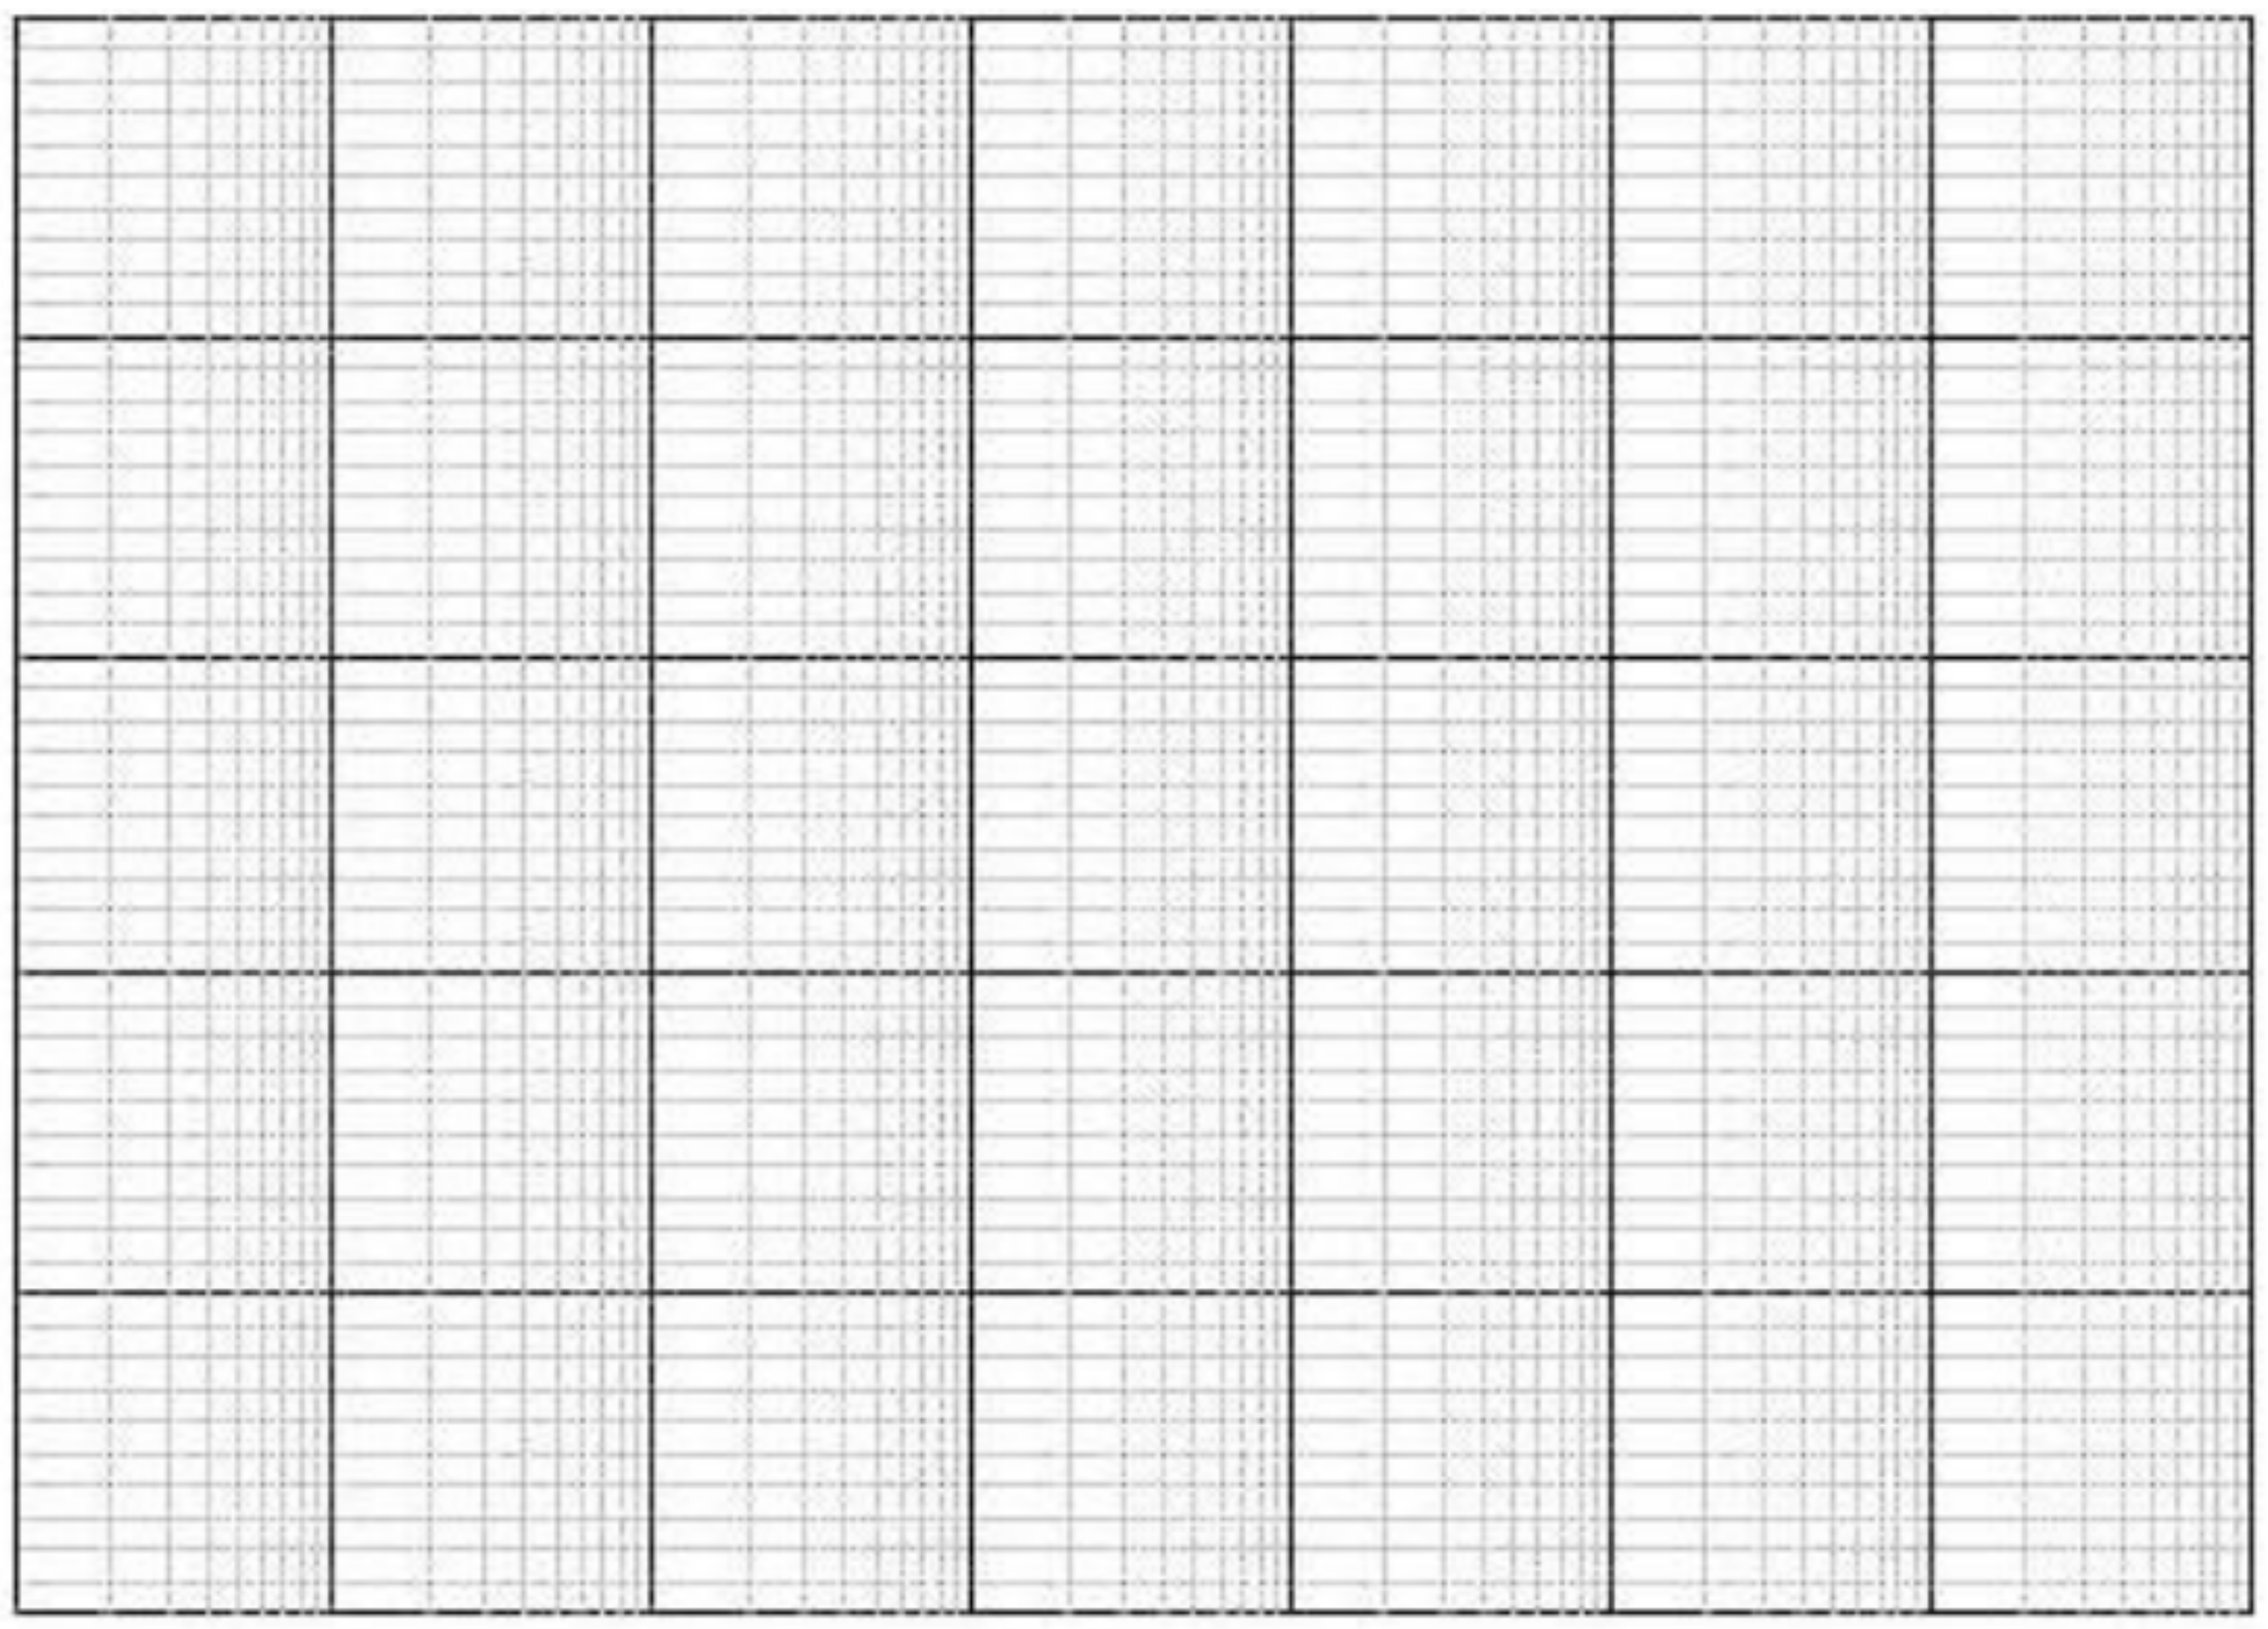
\includegraphics[width=1.0\textwidth]{\bank/transfer/figures/bodeblank}
    \caption*{$|H_z(\omega)|$}
  \end{minipage}
  \hfill
  \begin{minipage}[b]{0.45\textwidth}
  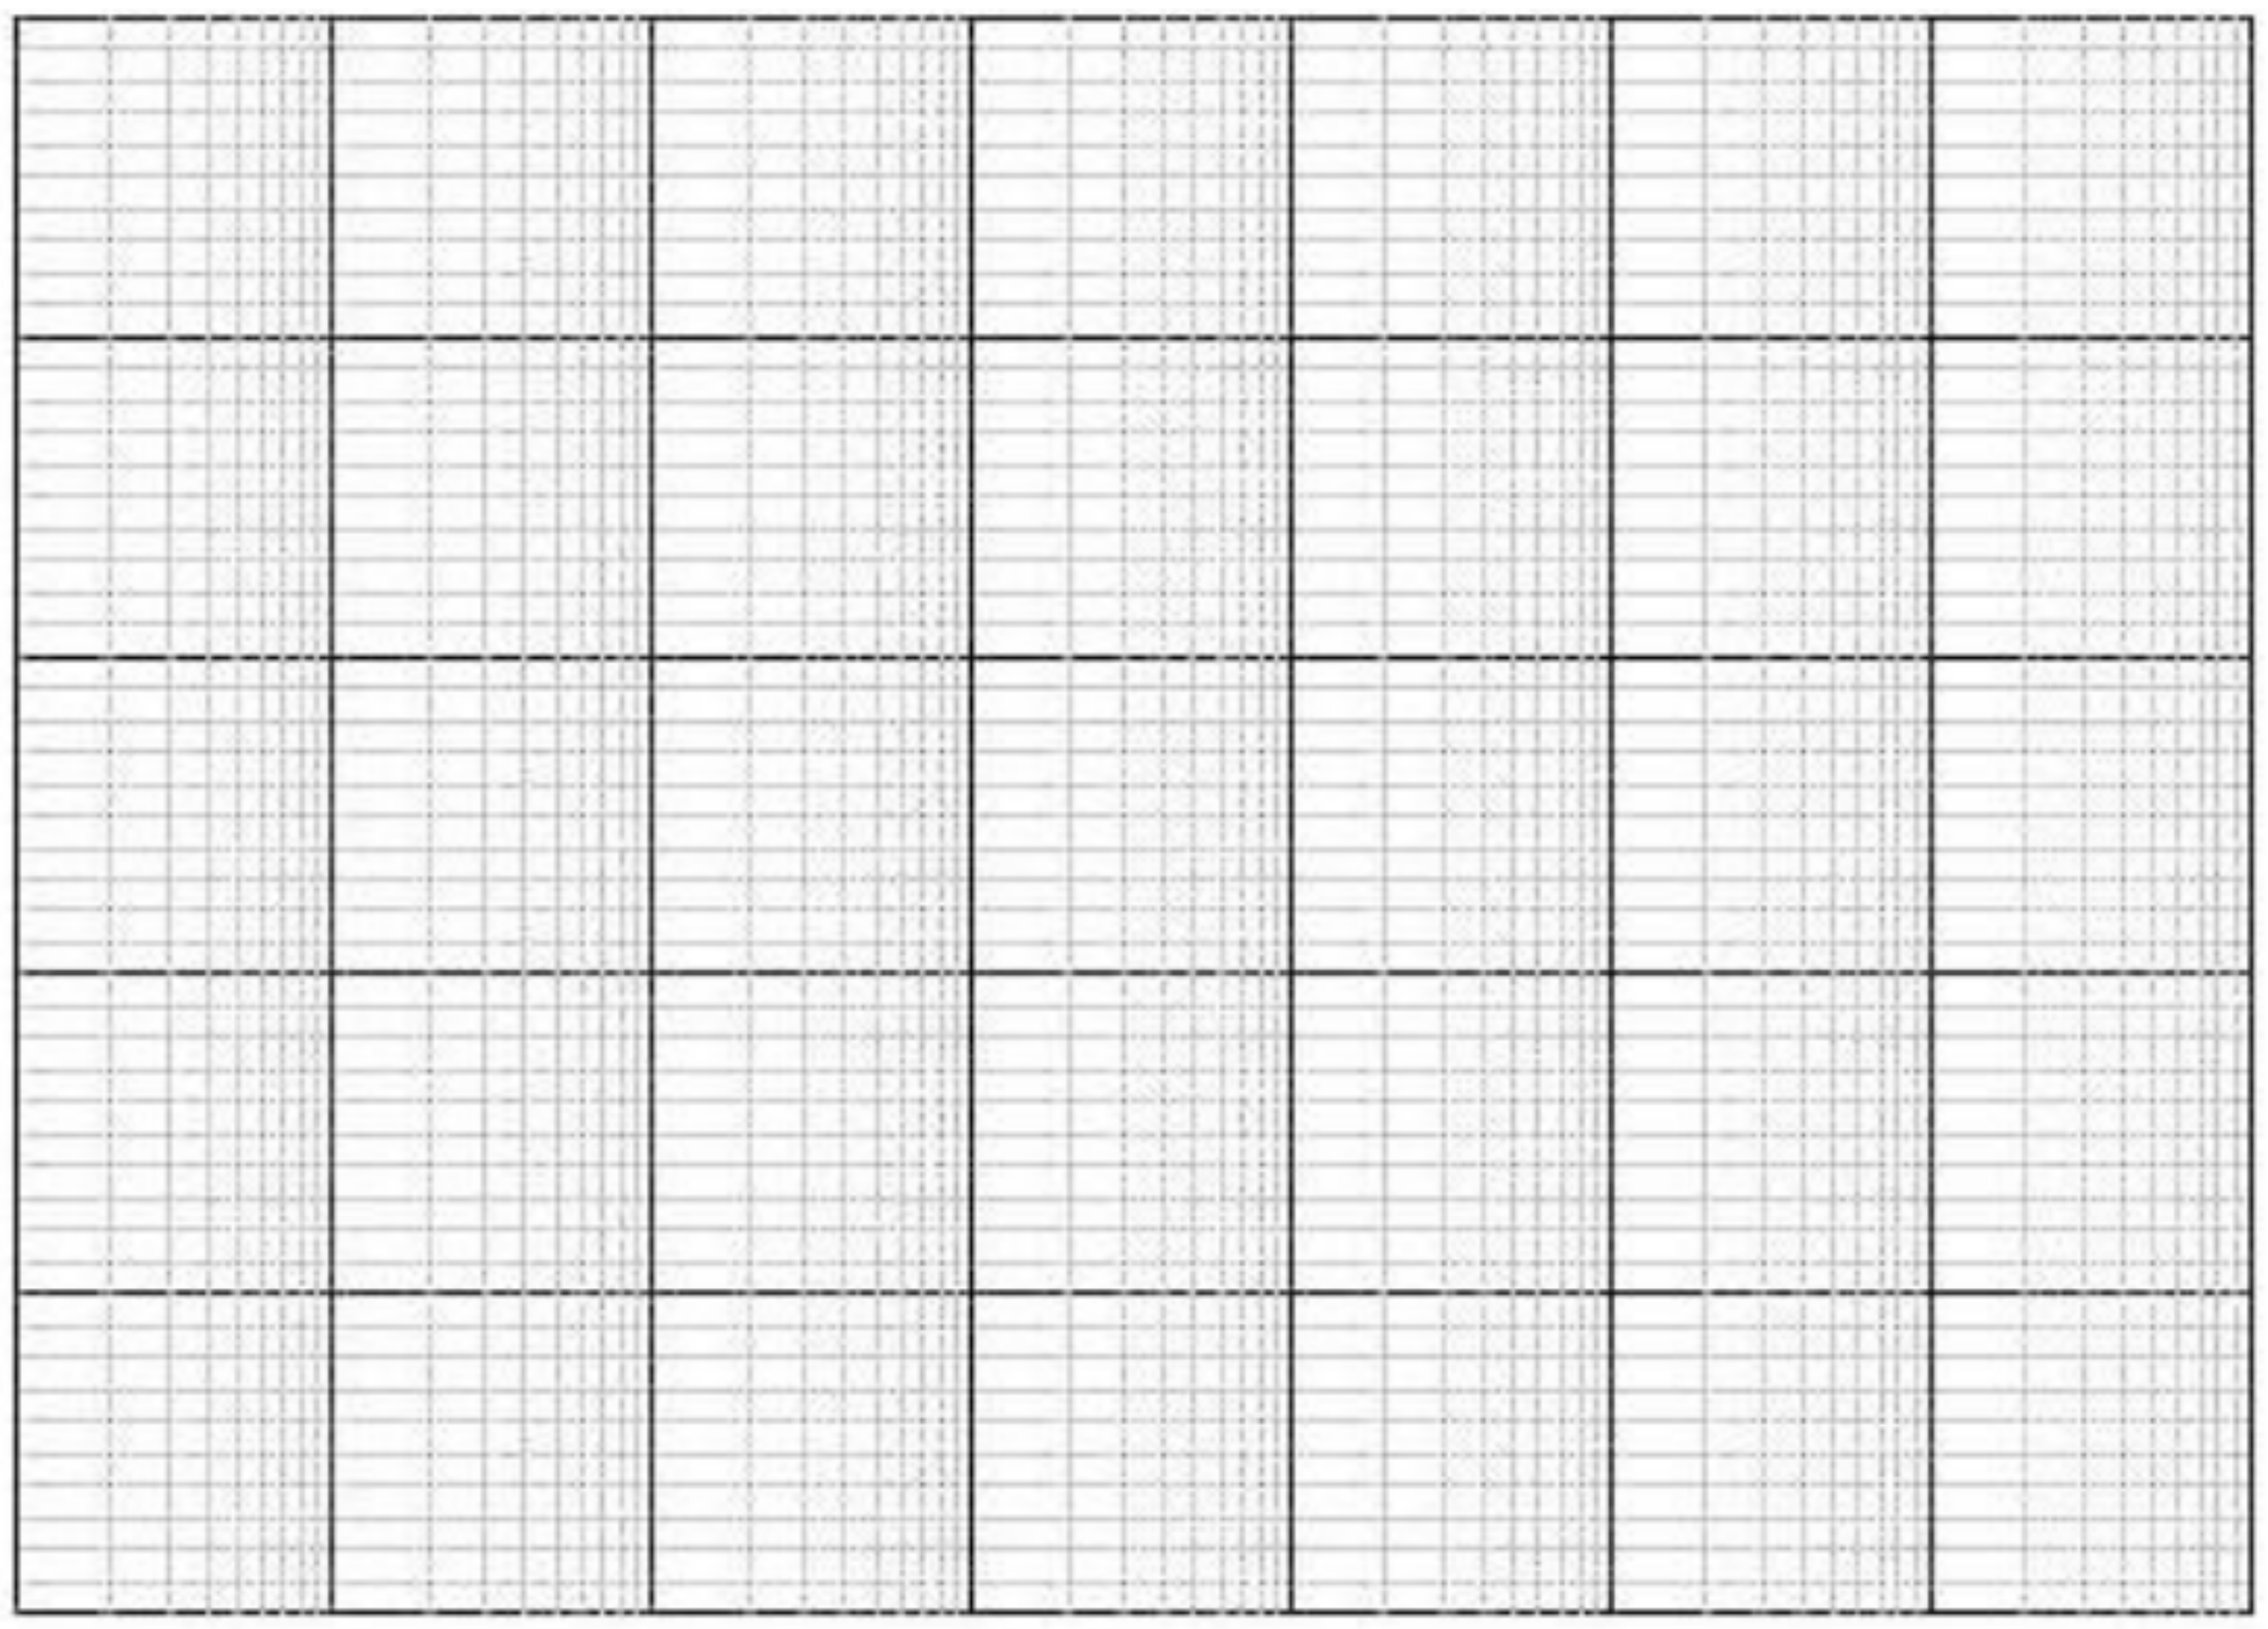
\includegraphics[width=1.0\textwidth]{\bank/transfer/figures/bodeblank}
    \caption*{$\angle H_z(\omega)$}
  \end{minipage}
\end{figure}

\sol{

  \begin{table}[h]
      \centering
      \begin{tabular}{| l | >{\centering\arraybackslash}m{6em} | >{\centering\arraybackslash}m{6em} | >{\centering\arraybackslash}m{6em} |} 
      \cline{2-4}
      \multicolumn{1}{l|}{}& $\omega << \omega_z$ & $\omega = \omega_z$ & $\omega >> \omega_z$ \\
      \hline
      &&&\\
      $H_z(\omega)$        &   1                 &       $1 + j$              &         $j \omega / \omega_z $           \\
      &&&\\
      \hline
      &&&\\
      $|H_z(\omega)|$      &   1                   &      $\sqrt{2} $              &      $\omega / \omega_z$                \\
      &&&\\
      \hline
      &&&\\
      $\angle H_z(\omega)$ &   0                   &      $\pi / 4$               &    $ \pi / 2$                  \\
      &&&\\
      \hline
      \end{tabular}
    \end{table}


\begin{figure}[!h]
  \centering
  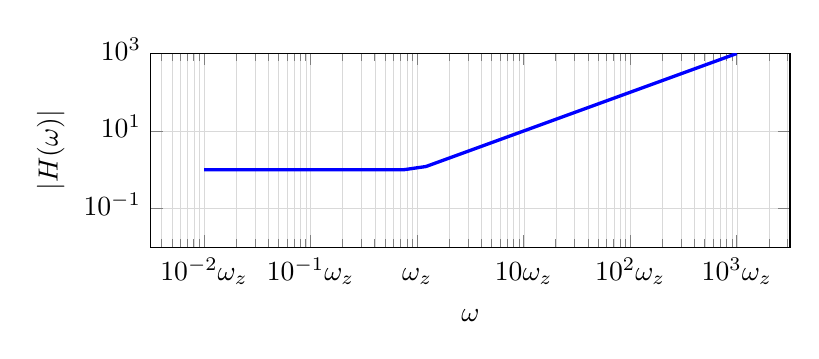
\begin{tikzpicture}[
      declare function={
        mag(\omega)= (\omega <= 10^2) * (1) +
                  (\omega > 10^2) * (\omega / 10^2)
       ;
      }
  ]

  \begin{loglogaxis}[
    typeset ticklabels with strut,
    ymin=0.01, ymax=1000, ylabel=$|H(\omega)|$,
    xticklabels = {$10^{-3} \omega_{z}$, $10^{-2} \omega_{z}$, $10^{-1} \omega_{z}$,
    $\omega_{z}$, $10 \omega_{z}$, $10^{2} \omega_{z}$, $10^{3} \omega_{z}$}, xlabel=$\omega$,
    , 
    domain=10^0:10^5, 
    grid=both, grid style={line width=.1pt, draw=gray!30},
    width=\textwidth * 0.8,
    height=\textwidth / 3
  ]
  \addplot [blue,very thick] {mag(x)};
  \end{loglogaxis}
  \end{tikzpicture}

  \vspace{0.3 cm}

  \centering
  \hspace{0.9 cm}
  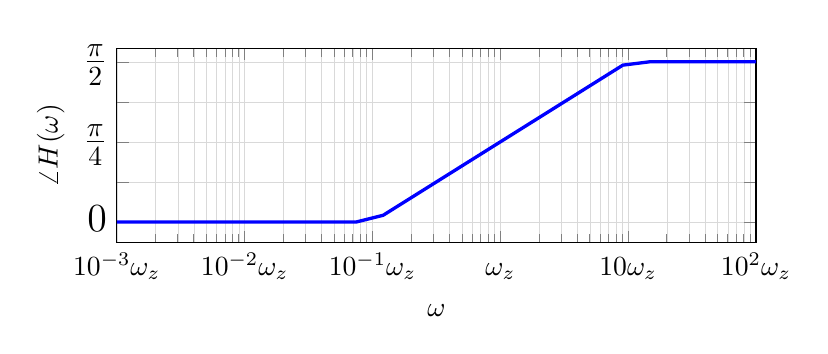
\begin{tikzpicture}[
      declare function={
        mag(\omega)= (\omega < 10^2) * (0) + and(\omega >= 10^2, \omega < 10^4) * (pi / 4 * (log10(\omega) - 2))
                  + (\omega >= 10^4) * (pi / 2)
       ;
      }
  ]
  \begin{semilogxaxis}[
    typeset ticklabels with strut,
    ymin=-0.2, ymax=1.7, ylabel=$\angle H(\omega)$, ytick={0, pi/8, pi/4, 3 * pi/8, pi/2}, 
    yticklabels={$0$, $\,$, $\frac{\pi}{4}$, $\,$, $\frac{\pi}{2}$},
    yticklabel style={font=\Large},
    xmin=10^0, xmax=10^5, xlabel=$\omega$,
    xticklabels = {$10^{-3} \omega_{z}$, $10^{-2} \omega_{z}$, $10^{-1} \omega_{z}$,
    $\omega_{z}$, $10 \omega_{z}$, $10^{2} \omega_{z}$}, 
    domain=10^0:10^5, 
    grid=both, grid style={line width=.1pt, draw=gray!30},
    width=\textwidth * 0.8,
    height=\textwidth / 3
  ]
  \addplot [blue,very thick] {mag(x)};
  \end{semilogxaxis}
  \end{tikzpicture}
\end{figure}

}

\qitem Let $H_p(\omega) = \frac{1}{1 + j \frac{\omega}{\omega_p}}$. This is called a \textbf{pole at $\omega_p$}, where $\omega_p$ is the \textbf{pole frequency}. Note that this is the reciprocal of the zero in the previous part.
\begin{enumerate}
    \qitem Find $|H_p(\omega)|$ and $\angle H_p(\omega)$.
    \qitem Again, \textbf{fill in the following table to analyze the magnitude and phase at the three regions $\omega << \omega_p$, $\omega = \omega_p$, and $\omega >> \omega_p$.}

    \begin{table}[ht!]
      \centering
      \begin{tabular}{| l | >{\centering\arraybackslash}m{6em} | >{\centering\arraybackslash}m{6em} | >{\centering\arraybackslash}m{6em} |} 
      \cline{2-4}
      \multicolumn{1}{l|}{}& $\omega << \omega_p$ & $\omega = \omega_p$ & $\omega >> \omega_p$ \\
      \hline
      &&&\\
      $H_p(\omega)$        &                      &                     &                      \\
      &&&\\
      \hline
      &&&\\
      $|H_p(\omega)|$      &                      &                     &                      \\
      &&&\\
      \hline
      &&&\\
      $\angle H_p(\omega)$ &                      &                     &                      \\
      &&&\\
      \hline
      \end{tabular}
    \end{table}

    \qitem \textbf{Plot the Bode plot for $|H_p(\omega)|$ and $\angle H_p(\omega)$.}
           Use the same way of approximating as described in the previous part.
\end{enumerate}

\begin{figure}[h]
  \centering
  \begin{minipage}[b]{0.45\textwidth}
  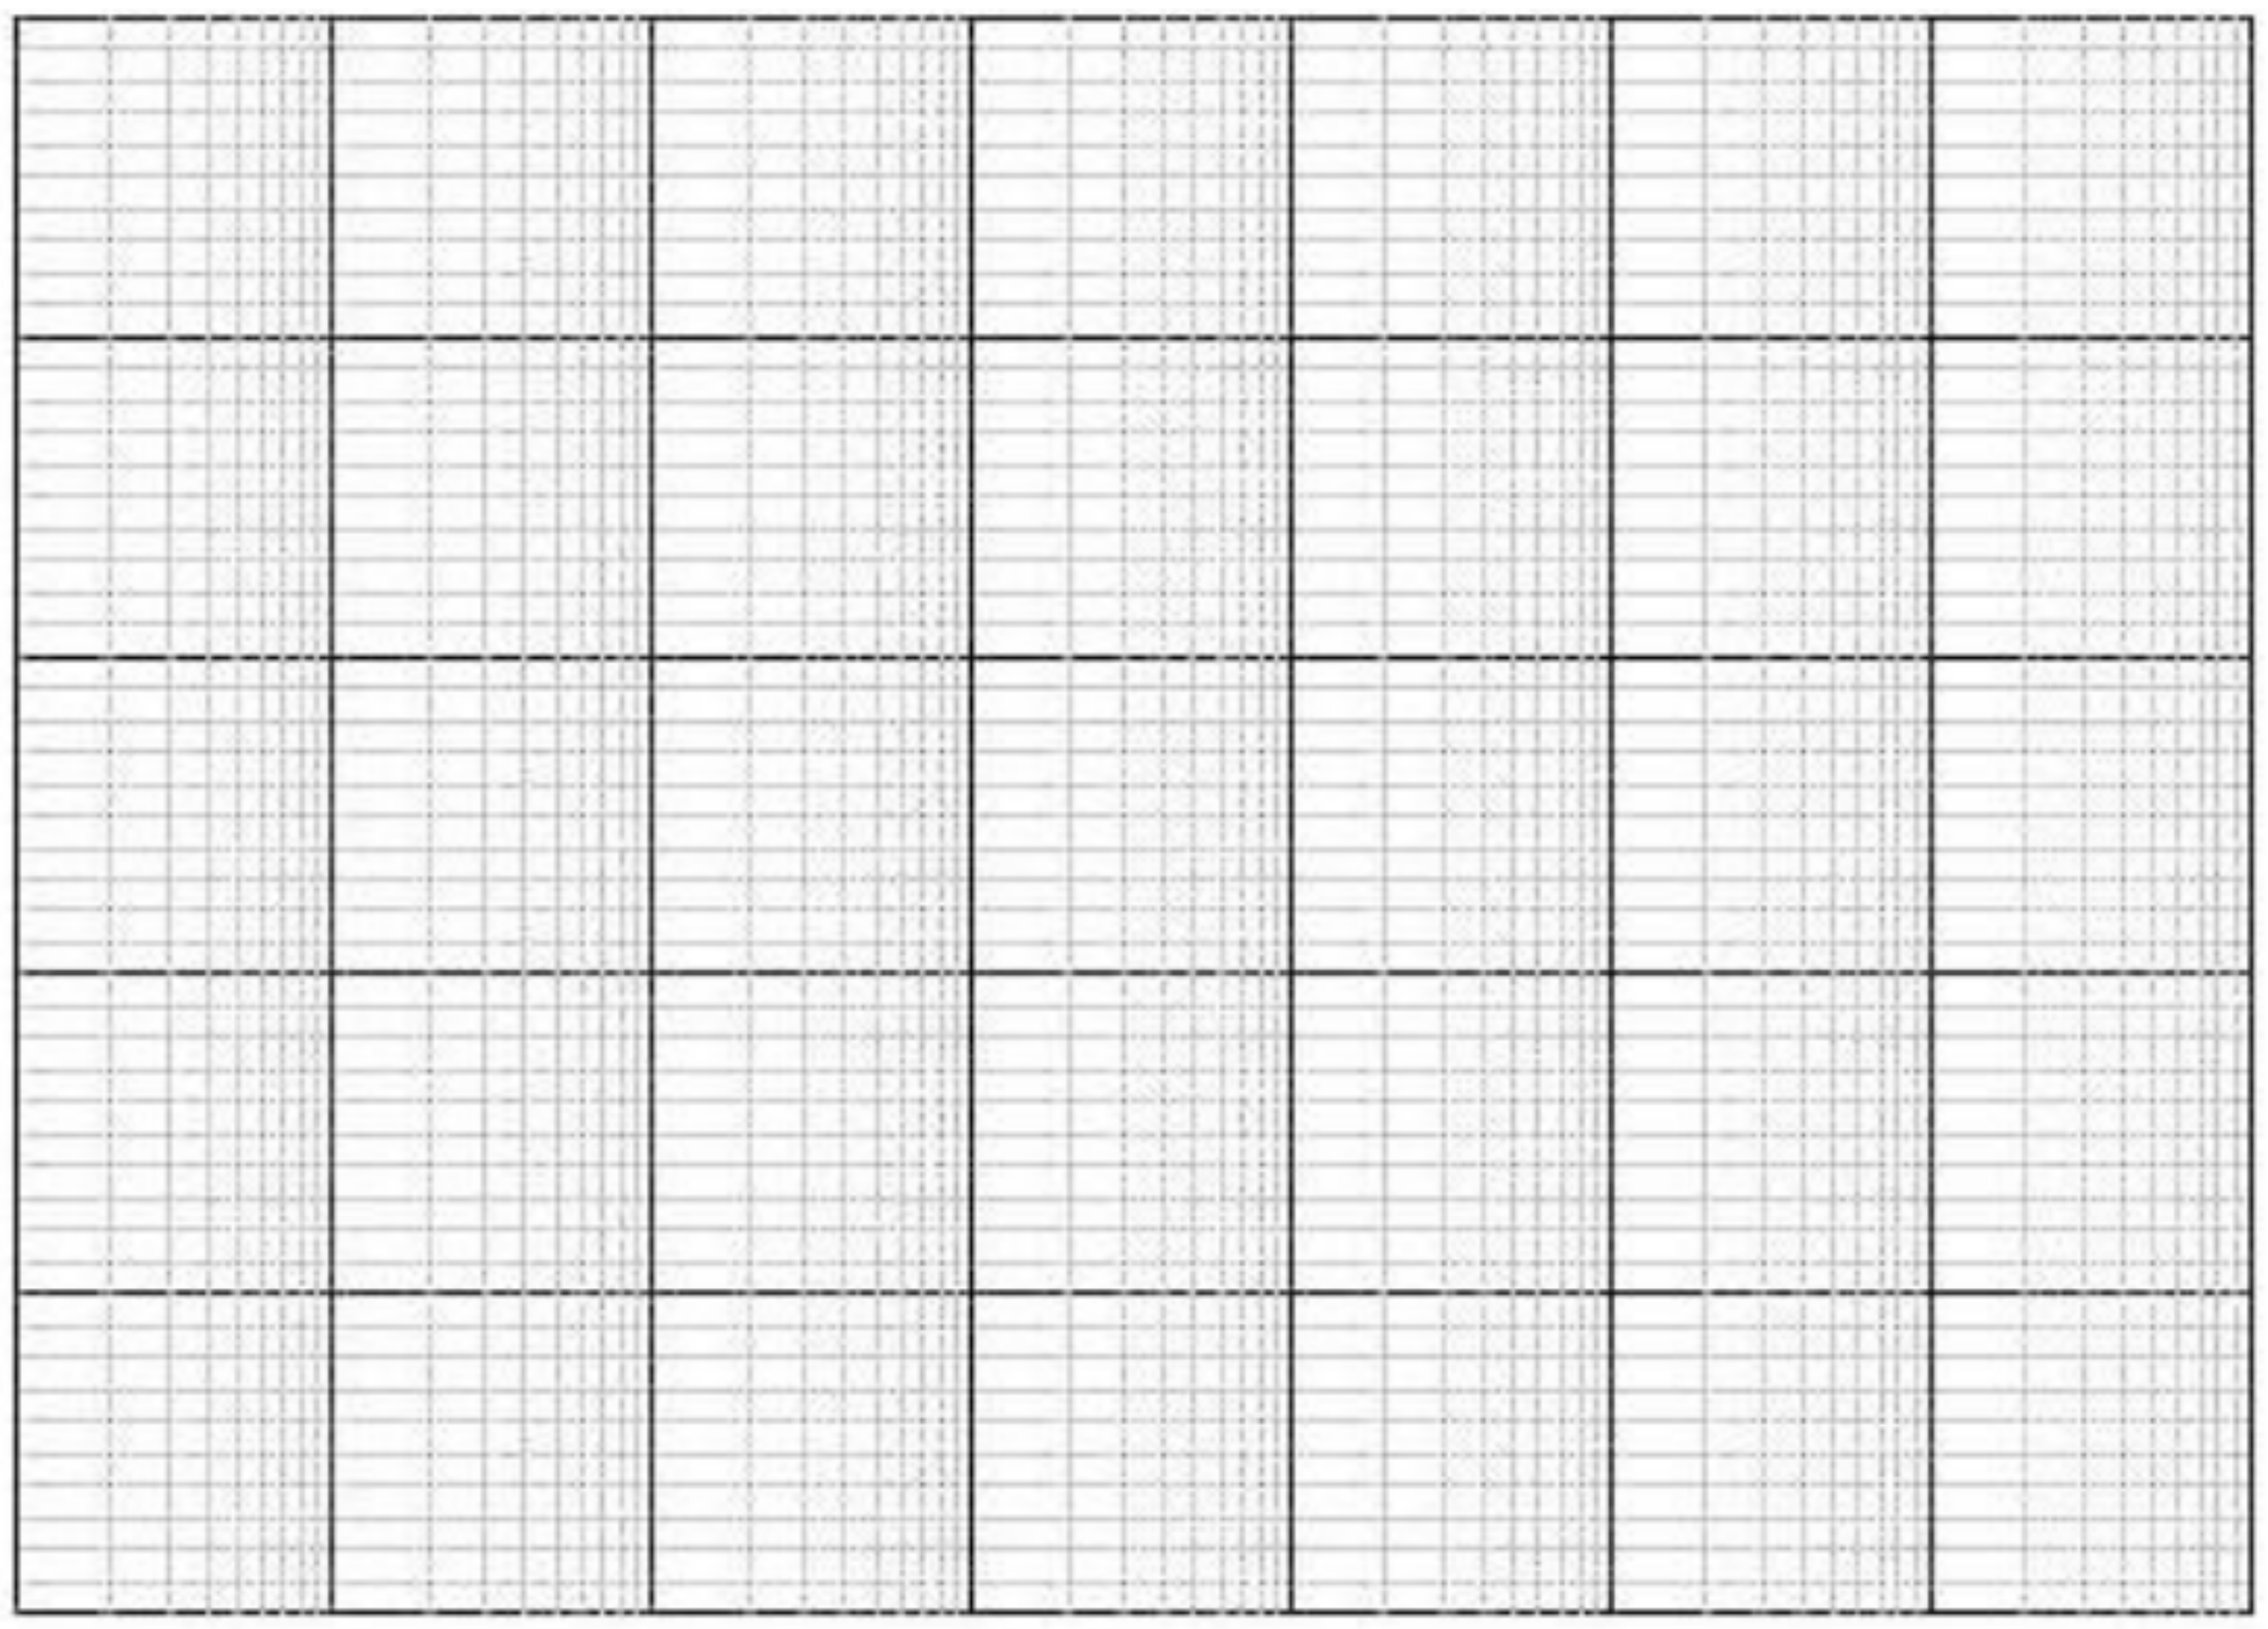
\includegraphics[width=1.0\textwidth]{\bank/transfer/figures/bodeblank}
    \caption*{$|H_z(\omega)|$}
  \end{minipage}
  \hfill
  \begin{minipage}[b]{0.45\textwidth}
  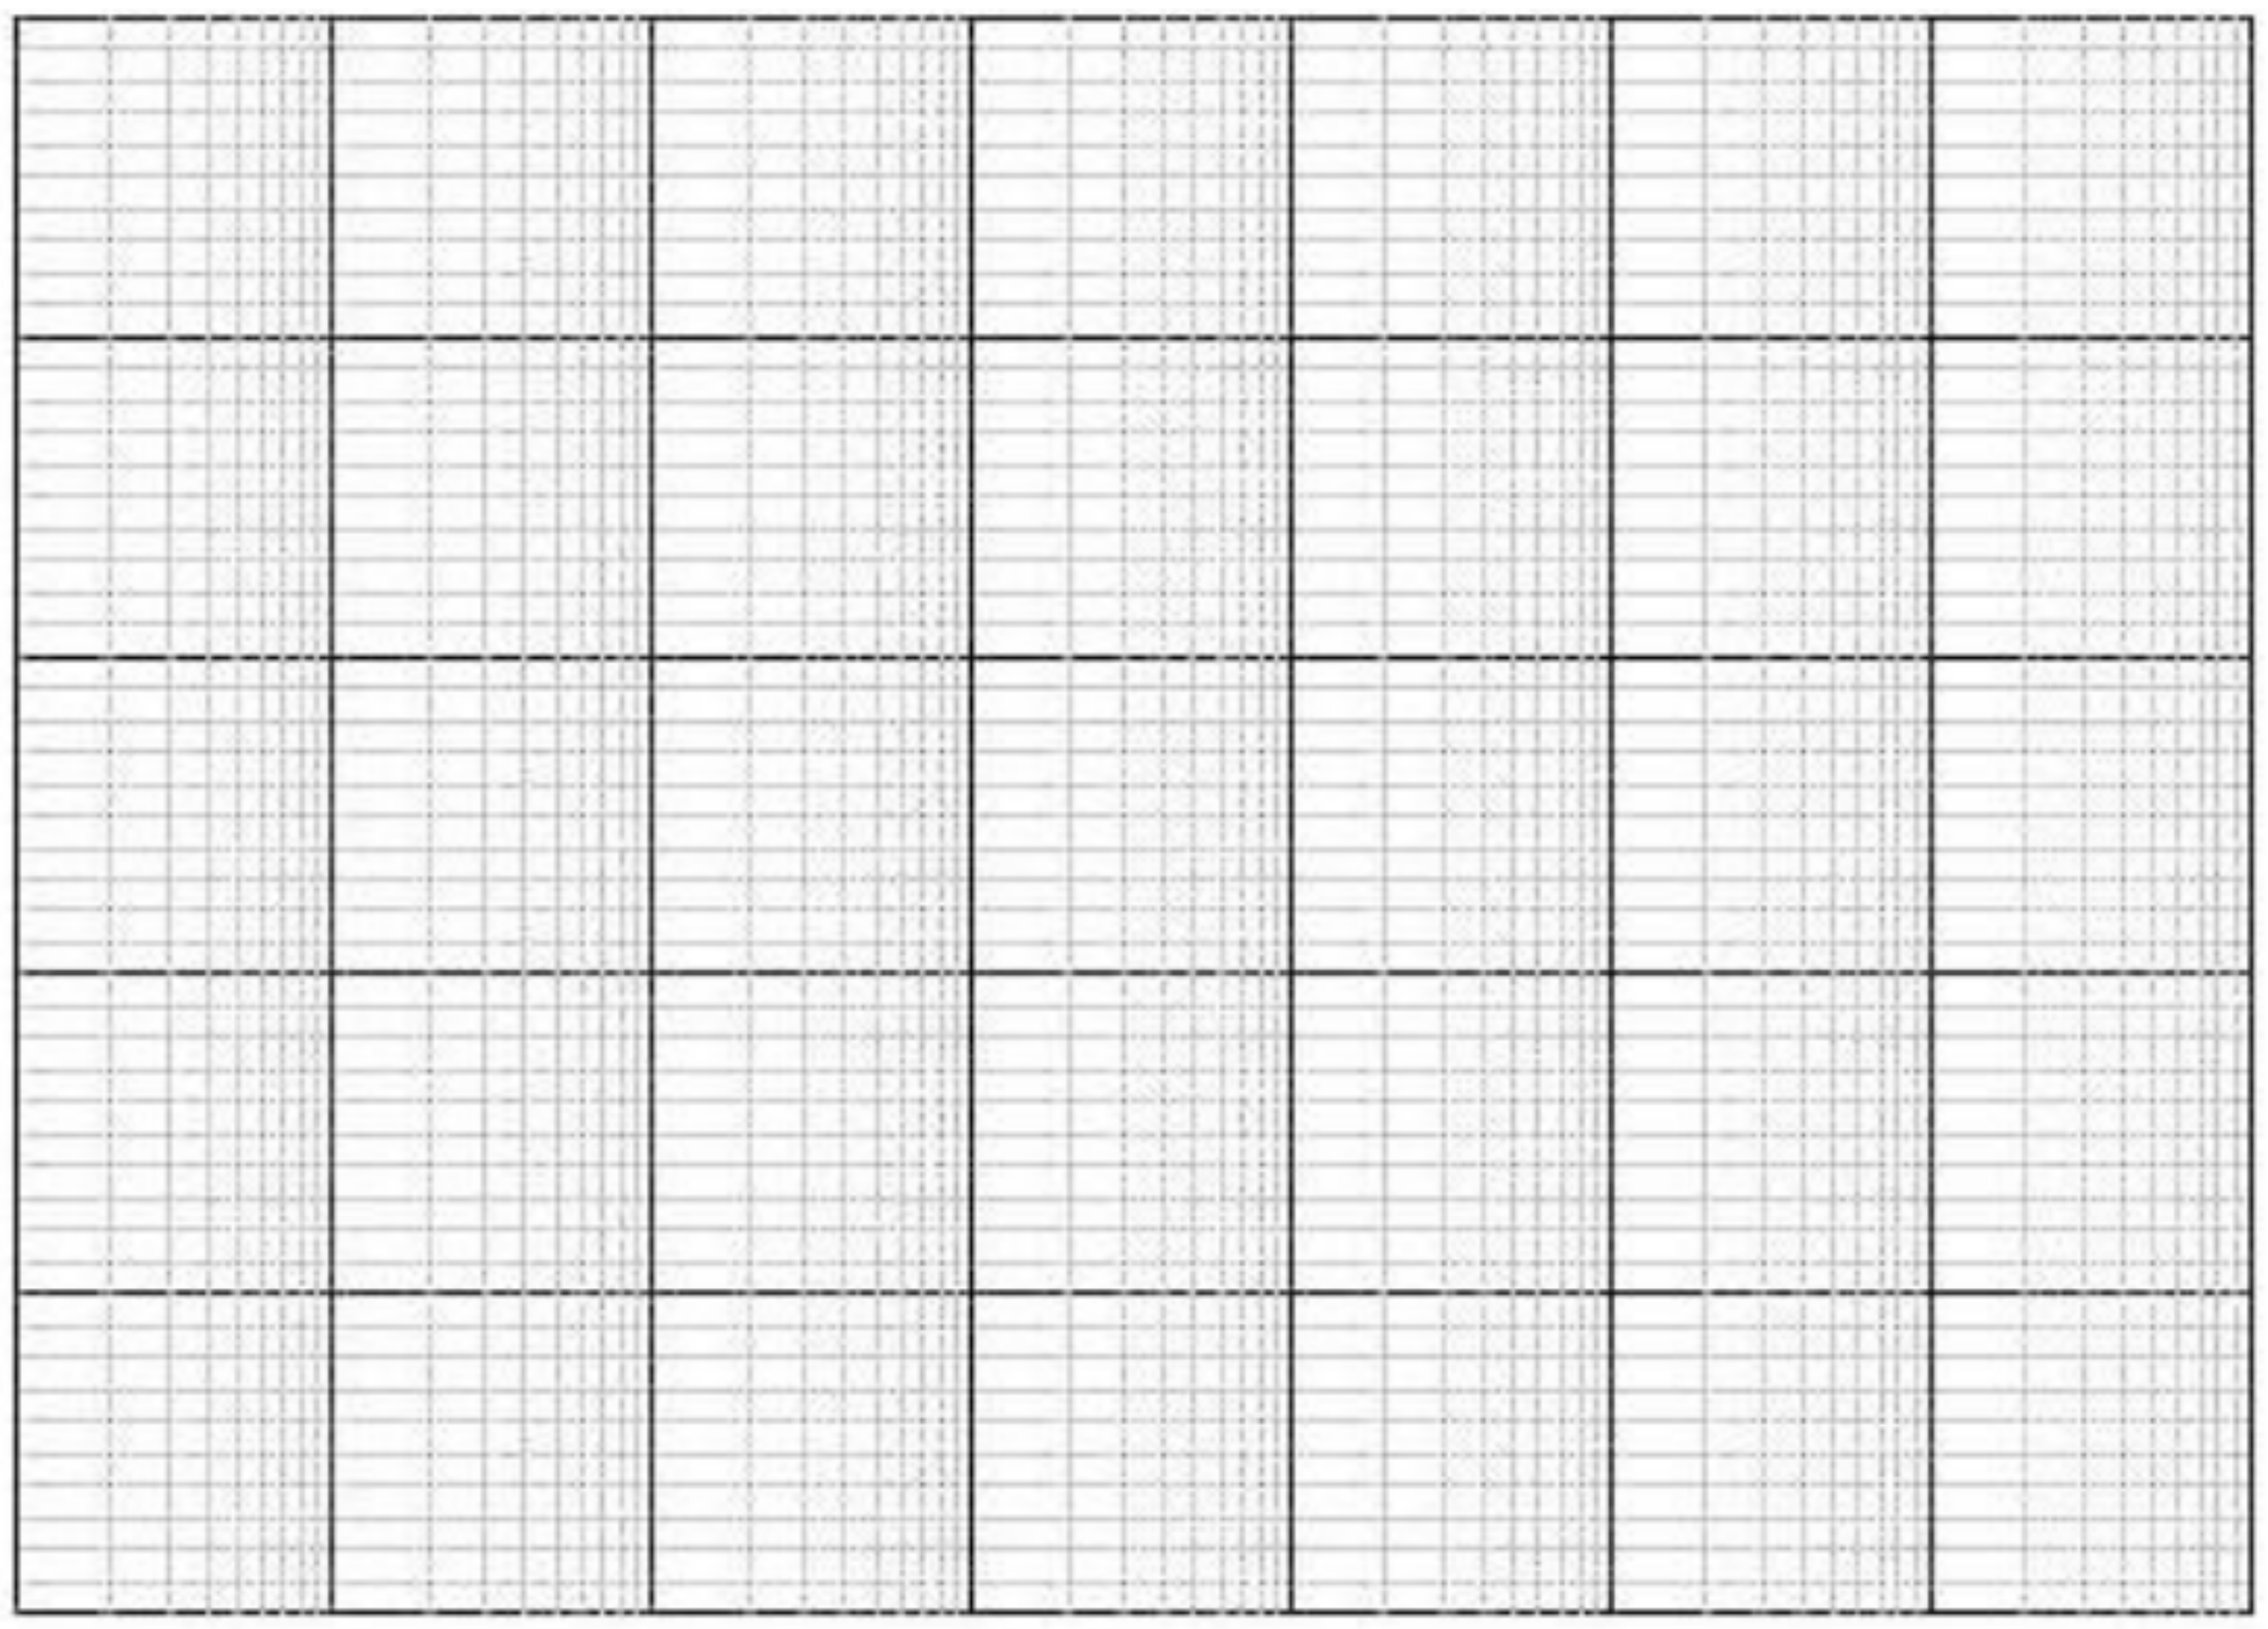
\includegraphics[width=1.0\textwidth]{\bank/transfer/figures/bodeblank}
    \caption*{$\angle H_z(\omega)$}
  \end{minipage}
\end{figure}

\sol{
\newpage
\begin{figure}[h]
  \centering
  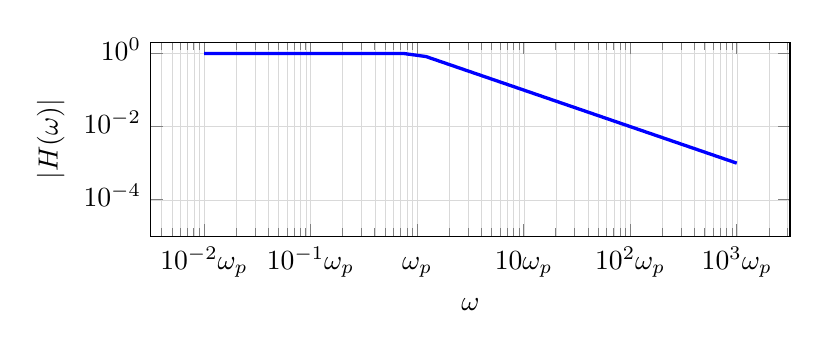
\begin{tikzpicture}[
      declare function={
        mag(\omega)= (\omega < 10^2) * (1) +
                  (\omega >= 10^2) * (10^2 / \omega)
       ;
      }
  ]
  \begin{loglogaxis}[
    typeset ticklabels with strut,
    ymin=0.00001, ymax=2, ylabel=$|H(\omega)|$,
    xticklabels = {$10^{-3} \omega_{p}$, $10^{-2} \omega_{p}$, $10^{-1} \omega_{p}$,
    $\omega_{p}$, $10 \omega_{p}$, $10^{2} \omega_{p}$, $10^{3} \omega_{p}$}, xlabel=$\omega$,
    , 
    domain=10^0:10^5, 
    grid=both, grid style={line width=.1pt, draw=gray!30},
    width=\textwidth * 0.8,
    height=\textwidth / 3
  ]
  \addplot [blue,very thick] {mag(x)};
  \end{loglogaxis}
  \end{tikzpicture}

  \vspace{0.3 cm}

  \centering
  \hspace{0.9 cm}
  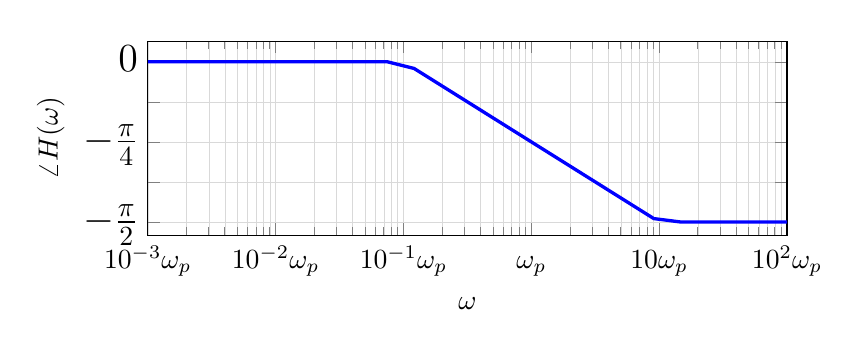
\begin{tikzpicture}[
      declare function={
        mag(\omega)= (\omega < 10^2) * (0) + and(\omega >= 10^2, \omega < 10^4) * (pi / 4 * (-log10(\omega) + 2))
                  + (\omega >= 10^4) * (-pi / 2)
       ;
      }
  ]
  \begin{semilogxaxis}[
    typeset ticklabels with strut,
    ymin=-1.7, ymax=0.2, ylabel=$\angle H(\omega)$, ytick={0, -pi/8, -pi/4, -3 * pi/8, -pi/2}, 
    yticklabels={$0$, $\,$, $-\frac{\pi}{4}$, $\,$, $-\frac{\pi}{2}$},
    yticklabel style={font=\Large},
    xmin=10^0, xmax=10^5, xlabel=$\omega$,
    xticklabels = {$10^{-3} \omega_{p}$, $10^{-2} \omega_{p}$, $10^{-1} \omega_{p}$,
    $\omega_{p}$, $10 \omega_{p}$, $10^{2} \omega_{p}$}, 
    domain=10^0:10^5, 
    grid=both, grid style={line width=.1pt, draw=gray!30},
    width=\textwidth * 0.8,
    height=\textwidth / 3
  ]
  \addplot [blue,very thick] {mag(x)};
  \end{semilogxaxis}
  \end{tikzpicture}
\end{figure}
}

\qitem \textbf{What is the relationship between zero and poles (both graphically and algebraically)?}

\sol{

}

\qitem (Optional) Let $H_0(\omega) = j\omega$. This is called a \textbf{zero at the origin}.
\begin{enumerate}
  \qitem \textbf{Find $|H_0(\omega)|$ and $\angle H_0(\omega)$}.
  \qitem \textbf{Sketch them on the next page.}

\begin{figure}[!ht]
  \centering
  \begin{minipage}[b]{0.45\textwidth}
  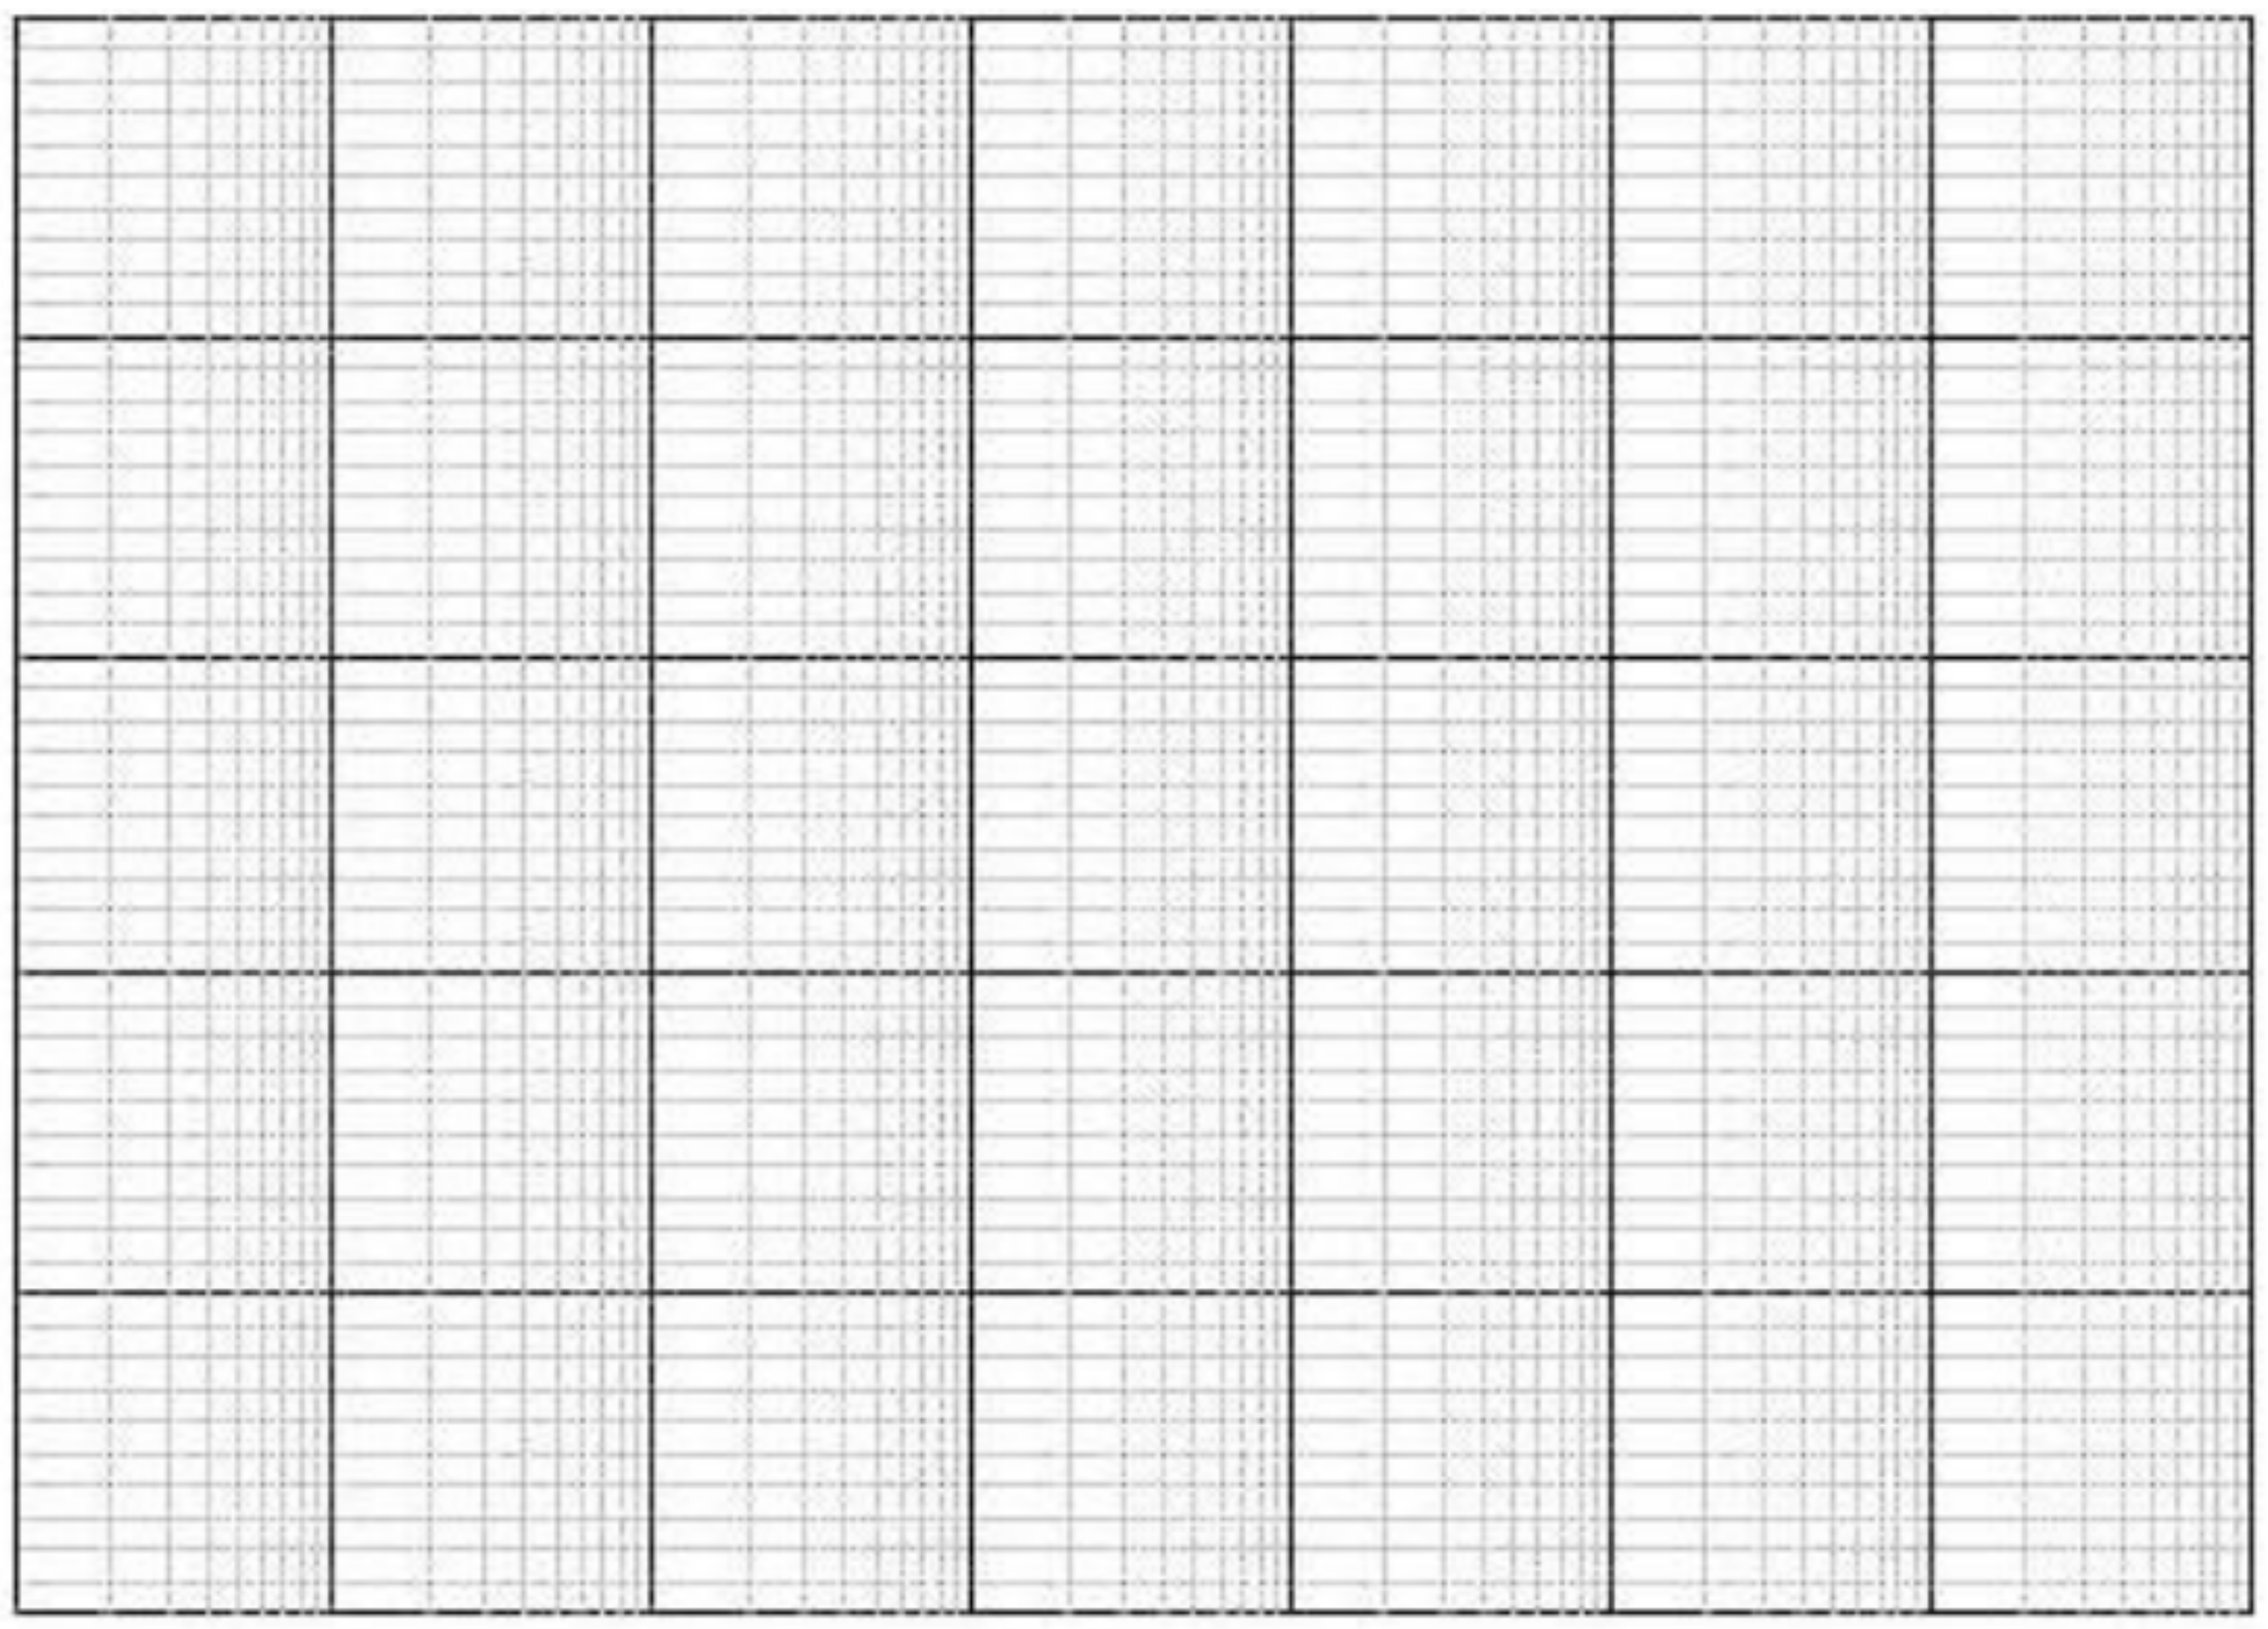
\includegraphics[width=1.0\textwidth]{\bank/transfer/figures/bodeblank}
    \caption*{$|H_0(\omega)|$}
  \end{minipage}
  \hfill
  \begin{minipage}[b]{0.45\textwidth}
  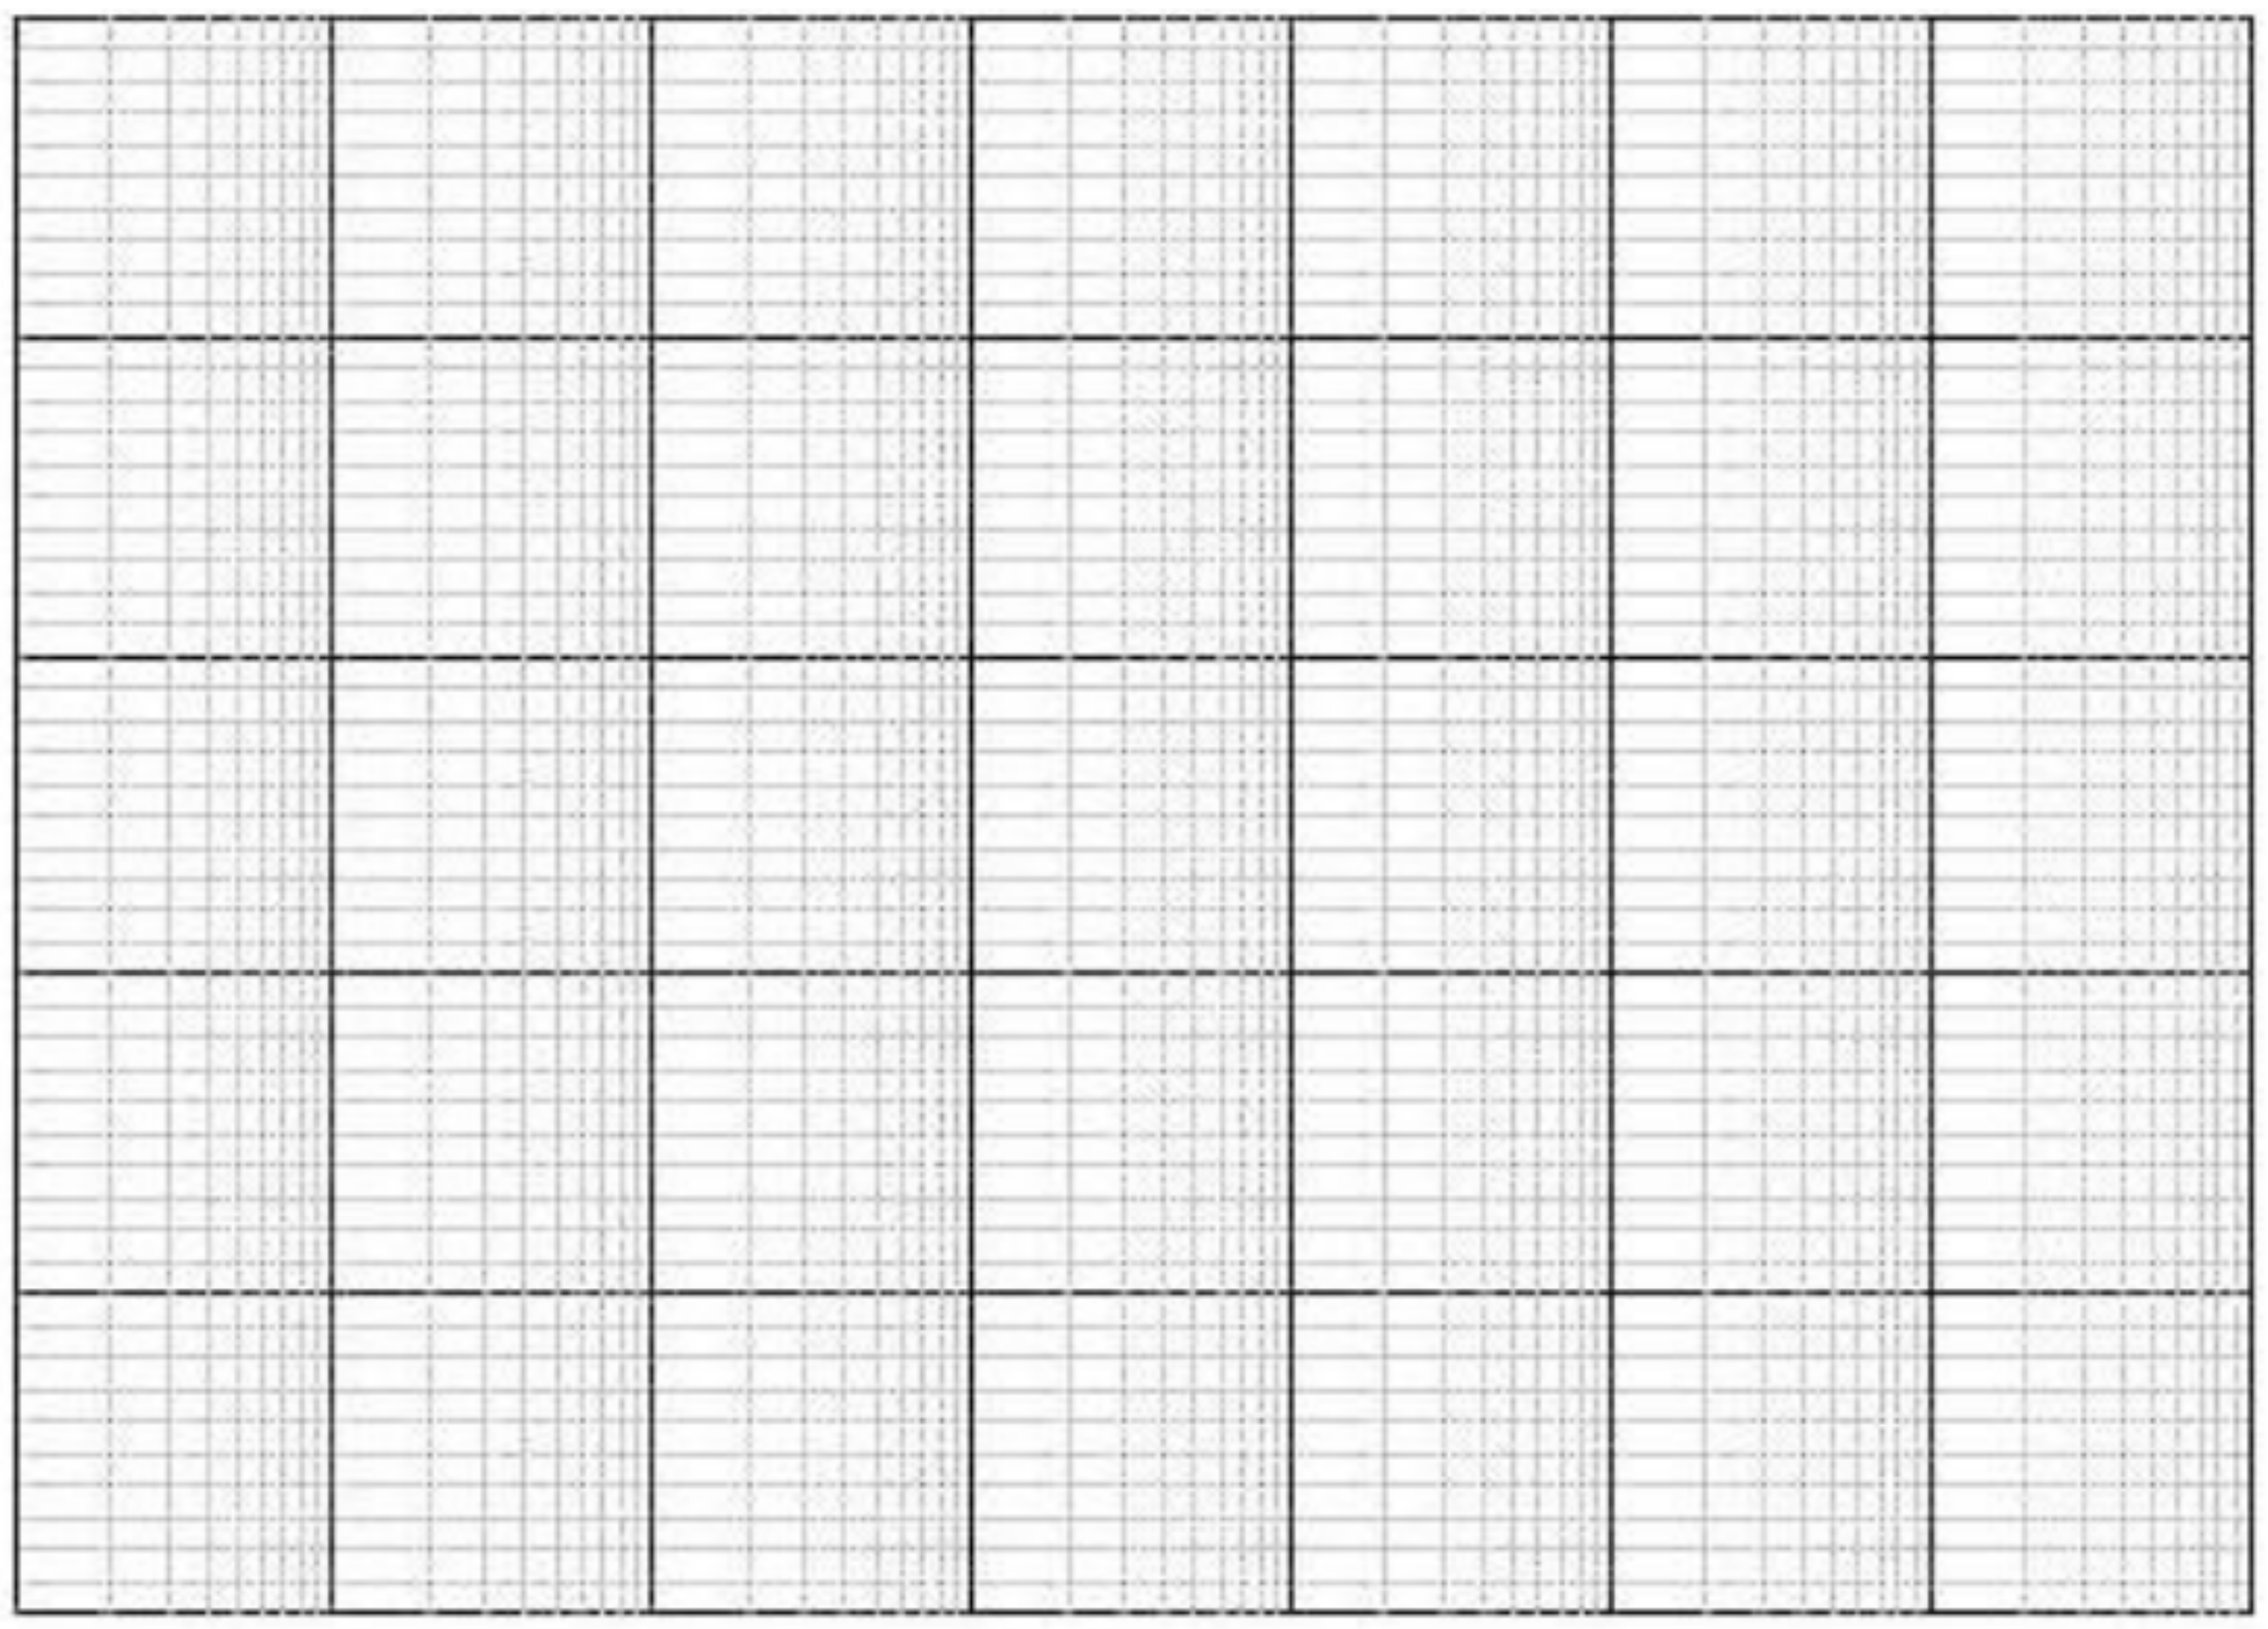
\includegraphics[width=1.0\textwidth]{\bank/transfer/figures/bodeblank}
    \caption*{$\angle H_0(\omega)$}
  \end{minipage}
\end{figure}
\end{enumerate}

\sol{
\begin{figure}[!ht]
  \centering
  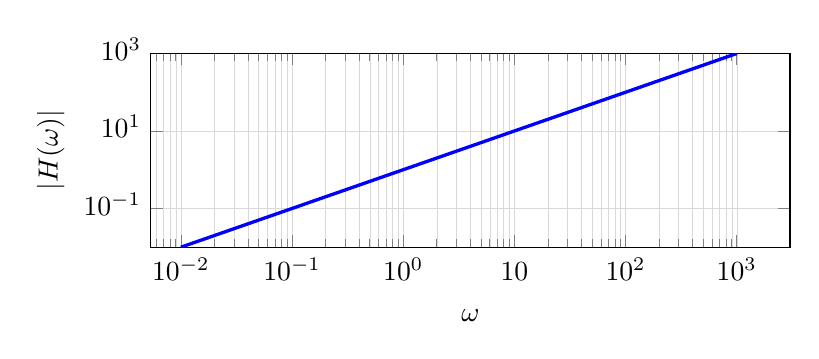
\begin{tikzpicture}[
      declare function={
        mag(\omega)= \omega
       ;
      }
  ]
  \begin{loglogaxis}[
    typeset ticklabels with strut,
    ymin=0.01, ymax=1000, ylabel=$|H(\omega)|$,
    xticklabels = {$10^{-3}$, $10^{-2}$, $10^{-1}$,
    $10^{0}$, $10$, $10^{2}$, $10^{3}$}, xlabel=$\omega$,
    , 
    domain=10^-2:10^3, 
    grid=both, grid style={line width=.1pt, draw=gray!30},
    width=\textwidth * 0.8,
    height=\textwidth / 3
  ]
  \addplot [blue,very thick] {mag(x)};
  \end{loglogaxis}
  \end{tikzpicture}

  \vspace{0.3 cm}

  \centering
  \hspace{0.9 cm}
  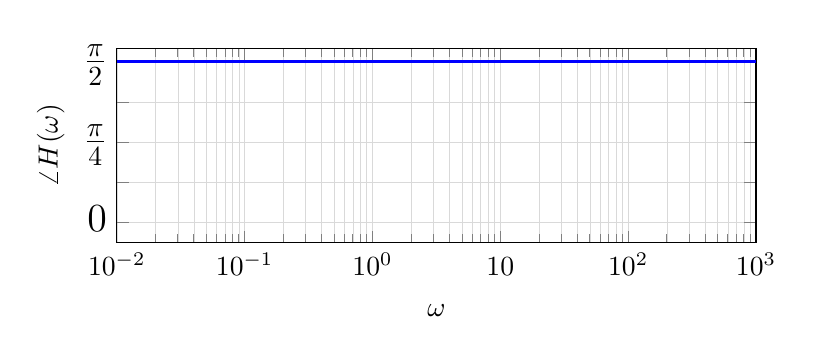
\begin{tikzpicture}[
      declare function={
        phase(\omega)= pi / 2
       ;
      }
  ]

  \begin{semilogxaxis}[
    typeset ticklabels with strut,
    ymin=-0.2, ymax=1.7, ylabel=$\angle H(\omega)$, ytick={0, pi/8, pi/4, 3 * pi/8, pi/2}, 
    yticklabels={$0$, $\,$, $\frac{\pi}{4}$, $\,$, $\frac{\pi}{2}$},
    yticklabel style={font=\Large},
    xmin=10^-2, xmax=10^3, xlabel=$\omega$,
    xticklabels = {$10^{-3}$, $10^{-2}$, $10^{-1}$,
    $10^{0}$, $10$, $10^{2}$, $10^{3}$}, 
    domain=10^-2:10^3, 
    grid=both, grid style={line width=.1pt, draw=gray!30},
    width=\textwidth * 0.8,
    height=\textwidth / 3
  ]
  \addplot [blue,very thick] {phase(x)};
  \end{semilogxaxis}
  \end{tikzpicture}
\end{figure}

}

\qitem (Optional) Let $H_1(\omega) = \frac{1}{j\omega}$. This is called a \textbf{pole at the origin}.
\begin{enumerate}
  \qitem \textbf{Find $|H_1(\omega)|$ and $\angle H_1(\omega)$}. What are these in terms of $|H_0(\omega)|$ and $\angle H_0(\omega)$?
  \qitem \textbf{Sketch $|H_1(\omega)|$ and $\angle H_1(\omega)$ on the next page.}
\end{enumerate}

\begin{figure}[!ht]
  \centering
  \begin{minipage}[b]{0.45\textwidth}
  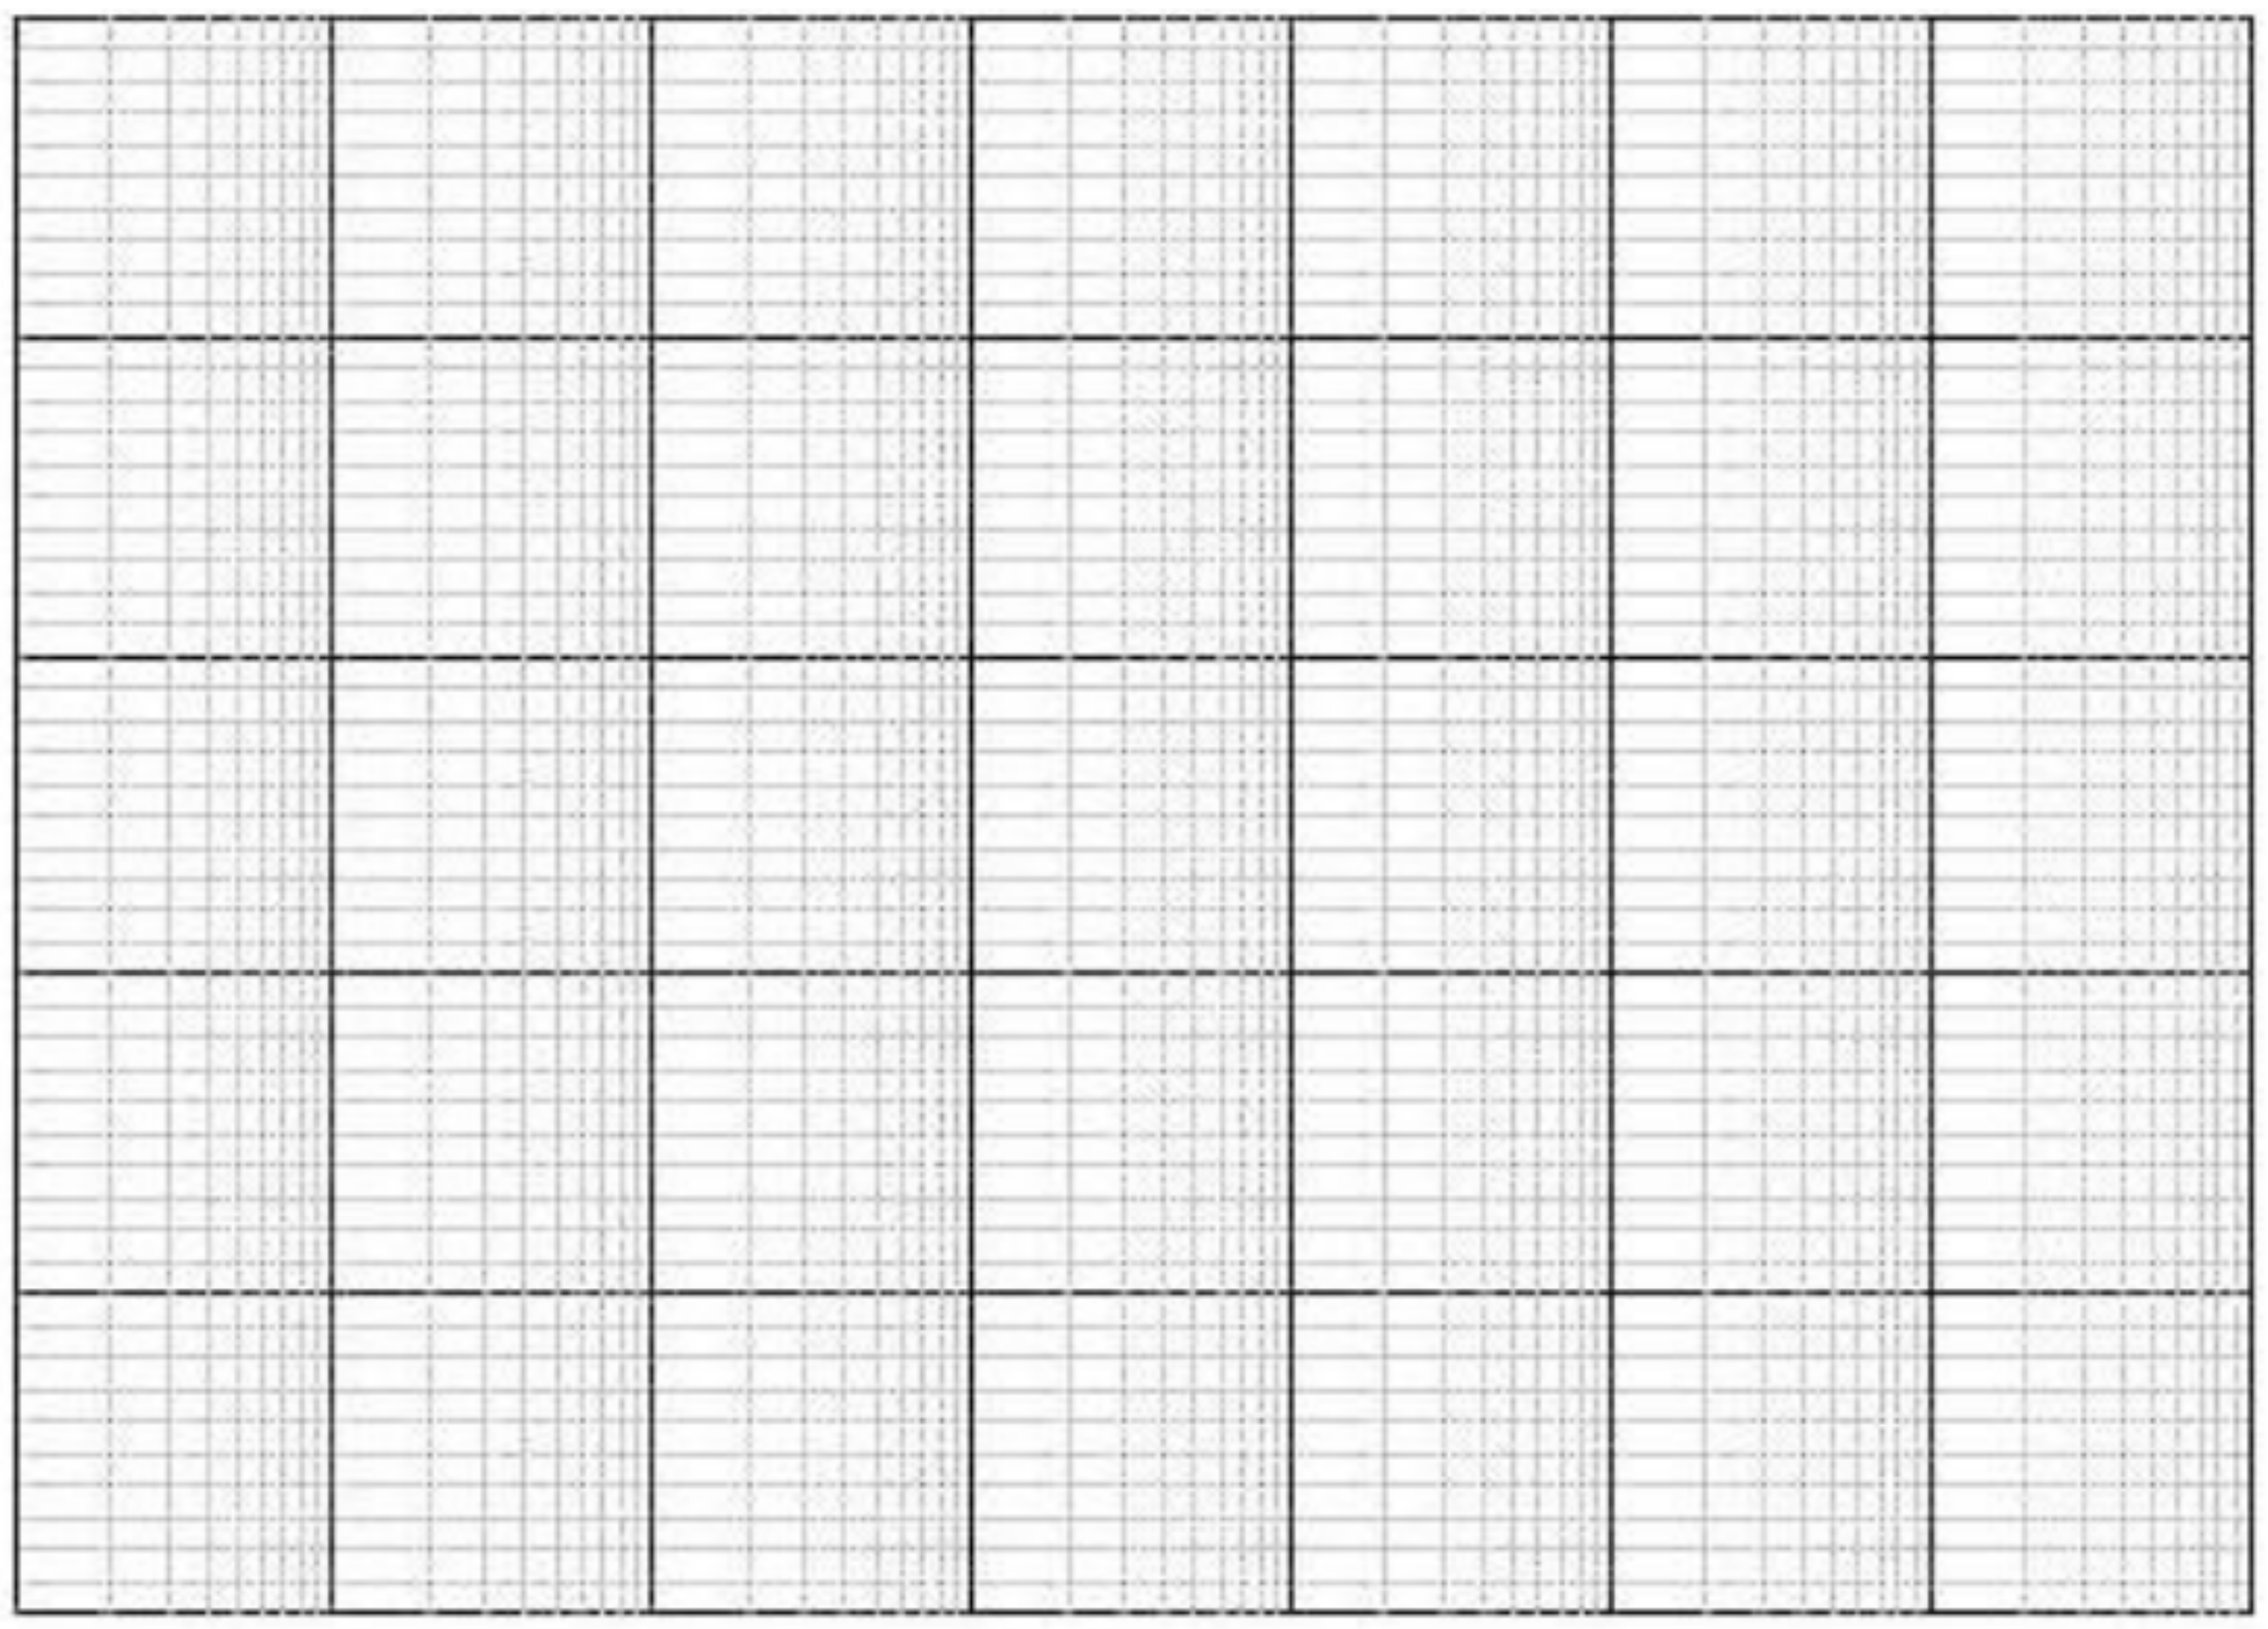
\includegraphics[width=1.0\textwidth]{\bank/transfer/figures/bodeblank}
    \caption*{$|H_1(\omega)|$}
  \end{minipage}
  \hfill
  \begin{minipage}[b]{0.45\textwidth}
  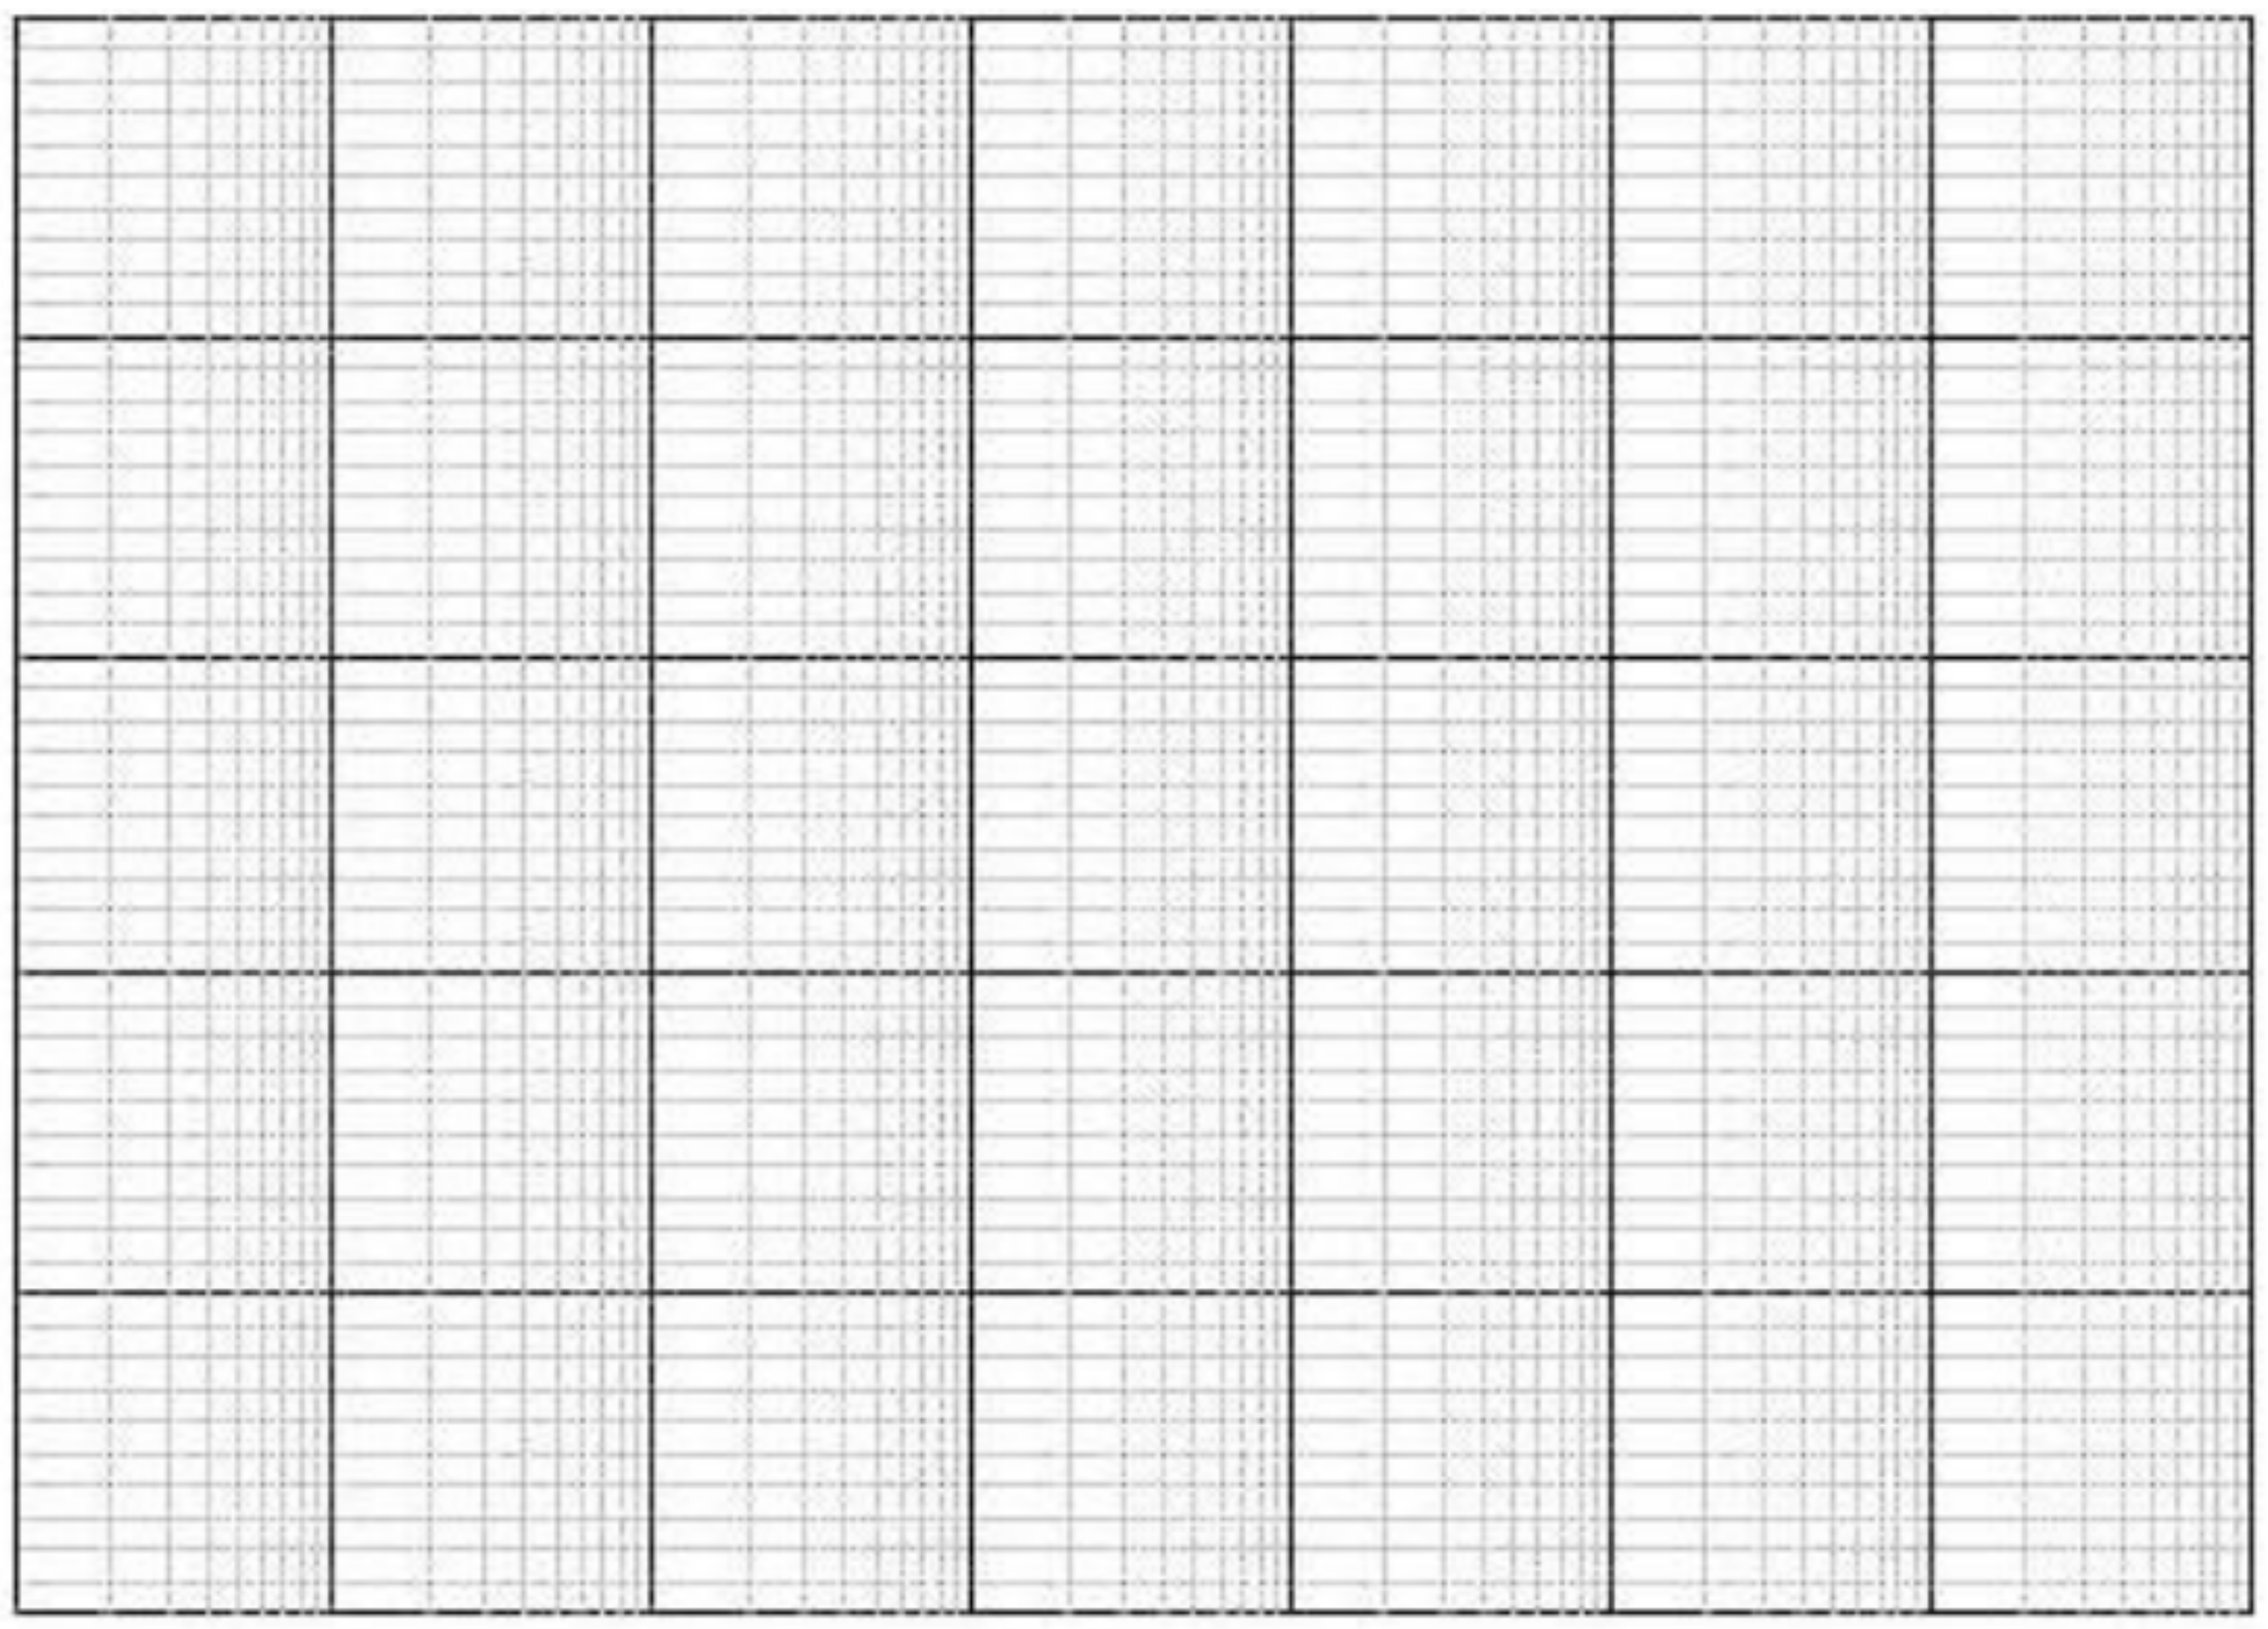
\includegraphics[width=1.0\textwidth]{\bank/transfer/figures/bodeblank}
    \caption*{$\angle H_1(\omega)$}
  \end{minipage}
\end{figure}

\sol{
\begin{figure}[h]
  \centering
  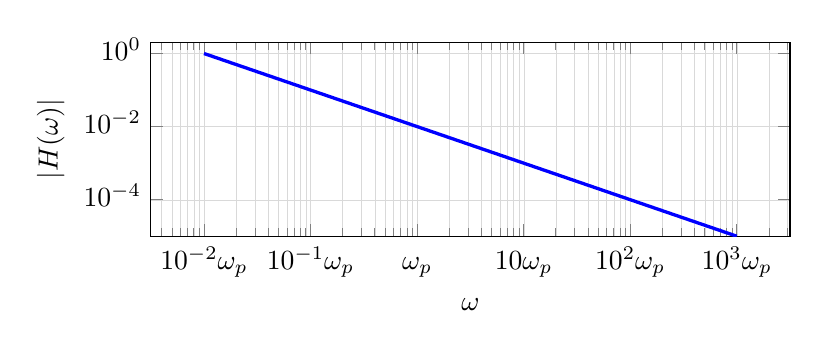
\begin{tikzpicture}[
      declare function={
        mag(\omega)= 1 / \omega
       ;
      }
  ]
  \begin{loglogaxis}[
    typeset ticklabels with strut,
    ymin=0.00001, ymax=2, ylabel=$|H(\omega)|$,
    xticklabels = {$10^{-3} \omega_{p}$, $10^{-2} \omega_{p}$, $10^{-1} \omega_{p}$,
    $\omega_{p}$, $10 \omega_{p}$, $10^{2} \omega_{p}$, $10^{3} \omega_{p}$}, xlabel=$\omega$,
    , 
    domain=10^0:10^5, 
    grid=both, grid style={line width=.1pt, draw=gray!30},
    width=\textwidth * 0.8,
    height=\textwidth / 3
  ]
  \addplot [blue,very thick] {mag(x)};
  \end{loglogaxis}
  \end{tikzpicture}

\end{figure}

\newpage

\begin{figure}[h]
  \vspace{0.3 cm}

  \centering
  \hspace{0.9 cm}
  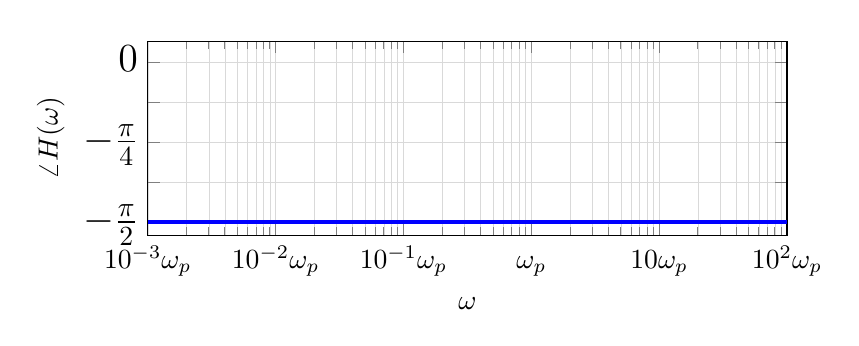
\begin{tikzpicture}[
      declare function={
        mag(\omega)= (-pi / 2)
       ;
      }
  ]
  \begin{semilogxaxis}[
    typeset ticklabels with strut,
    ymin=-1.7, ymax=0.2, ylabel=$\angle H(\omega)$, ytick={0, -pi/8, -pi/4, -3 * pi/8, -pi/2}, 
    yticklabels={$0$, $\,$, $-\frac{\pi}{4}$, $\,$, $-\frac{\pi}{2}$},
    yticklabel style={font=\Large},
    xmin=10^0, xmax=10^5, xlabel=$\omega$,
    xticklabels = {$10^{-3} \omega_{p}$, $10^{-2} \omega_{p}$, $10^{-1} \omega_{p}$,
    $\omega_{p}$, $10 \omega_{p}$, $10^{2} \omega_{p}$}, 
    domain=10^0:10^5, 
    grid=both, grid style={line width=.1pt, draw=gray!30},
    width=\textwidth * 0.8,
    height=\textwidth / 3
  ]
  \addplot [blue,very thick] {mag(x)};
  \end{semilogxaxis}
  \end{tikzpicture}
\end{figure}

}

\end{enumerate}
